% Template for a Computer Science Tripos Part II project dissertation
\documentclass[12pt,a4paper,twoside,openright]{report}
\usepackage[pdfborder={0 0 0}]{hyperref}    % turns references into hyperlinks
\usepackage[margin=25mm]{geometry}  % adjusts page layout
\usepackage{graphicx}  % allows inclusion of PDF, PNG and JPG images
\usepackage{docmute}   % only needed to allow inclusion of proposal.tex
\usepackage{listings}
\usepackage{tikz}
\usepackage{adjustbox}
\usepackage{multirow}

% tikz settings
\usetikzlibrary{shapes, arrows}

\raggedbottom                           % try to avoid widows and orphans
\sloppy
\clubpenalty1000%
\widowpenalty1000%

\renewcommand{\baselinestretch}{1.1}    % adjust line spacing to make
                                        % more readable

\definecolor{keywords}{RGB}{220,0,90}
\definecolor{strings}{RGB}{0,140,0}
\definecolor{comments}{RGB}{0,127,0}
\definecolor{identifiers}{RGB}{20,20,75}

\lstset{basicstyle=\ttfamily,
        keywordstyle=\color{keywords},
        commentstyle=\color{comments},
        stringstyle=\color{strings},
        showstringspaces=false,
        % identifierstyle=\color{identifiers},
        escapechar=$ %$
        }

\newcommand{\cbox}[2]{\adjustbox{bgcolor=#1}{#2}}

\begin{document}

\bibliographystyle{plain}


%%%%%%%%%%%%%%%%%%%%%%%%%%%%%%%%%%%%%%%%%%%%%%%%%%%%%%%%%%%%%%%%%%%%%%%%
% Title


\pagestyle{empty}

\rightline{\LARGE \textbf{Tianlin Zhang}}

\vspace*{60mm}
\begin{center}
\Huge
\textbf{An Observable OCaml} \\[5mm]
Computer Science Tripos -- Part II \\[5mm]
Jesus College \\[5mm]
\today  % today's date
\end{center}

%%%%%%%%%%%%%%%%%%%%%%%%%%%%%%%%%%%%%%%%%%%%%%%%%%%%%%%%%%%%%%%%%%%%%%%%%%%%%%
% Proforma, table of contents and list of figures

\pagestyle{plain}

\chapter*{Proforma}

{\large
\begin{tabular}{ll}
Name:               & \bf Tianlin Zhang \\
College:            & \bf Jesus College\\
Project Title:      & \bf An Observable OCaml\\
Examination:        & \bf Computer Science Tripos -- Part II, June 2018  \\
Word Count:         & \bf TODO\footnotemark[1]  \\
Project Originator: & Stephen Kell \\
Supervisor:         & Stephen Kell \\ 
\end{tabular}
}
\footnotetext[1]{This word count was computed
by \texttt{detex diss.tex | tr -cd '0-9A-Za-z $\tt\backslash$n' | wc -w}
}
\stepcounter{footnote}


\section*{Original Aims of the Project}

To write a backend for the OCaml compiler that allows compilation from OCaml 
into C in such a way that it preserves so-called ``observability'', that is the 
ability to debug the generated C code, using GDB for example, in a similar 
fashion to debugging the original OCaml code. A library of test programs should 
be written to demonstrate the capabilities of the compiler, along with an 
evaluation into the performance and observability of the compiled code.

\section*{Work Completed}

I have written and completed a new backend for the OCaml compiler which can compile an admissible subset of OCaml, including a majority of the most commonly used features. A C runtime library has also been written to support the compilation of the resulting C output, as well as a library of test programs which are used in testing and evaluation of the compiler. An evaluation has also been performed investigating the execution times of the compiler with respect to the OCaml native compiler, and the observability of the compiled code with the OCaml bytecode compiler.
% TODO - expand

\section*{Special Difficulties}

None.
 
\newpage
\section*{Declaration}

I, Tianlin Zhang of Jesus College, being a candidate for Part II of the Computer
Science Tripos, hereby declare
that this dissertation and the work described in it are my own work,
unaided except as may be specified below, and that the dissertation
does not contain material that has already been used to any substantial
extent for a comparable purpose.

\bigskip
\leftline{Signed: Tianlin Zhang}

\medskip
\leftline{Date: \today}

\tableofcontents

%%%%%%%%%%%%%%%%%%%%%%%%%%%%%%%%%%%%%%%%%%%%%%%%%%%%%%%%%%%%%%%%%%%%%%%
% now for the chapters

\pagestyle{headings}

\chapter{Introduction}

My project concerns the creation of a new compiler for OCaml, a popular statically typed functional language in the ML family, into the C language in such a way as to be able to take advantage of debugging tools provided by the C toolchain. This property, henceforth referred to as ``observability'', refers to the ability to view the execution of the program through a debugger as if it was debugging an OCaml program.

I have successfully implemented a compiler for a core subset of the OCaml language in to C, which when compiled with a standard C compiler such as \texttt{gcc} or \texttt{clang} produces an executable that behaves identically to the output of the native OCaml compiler. Additionally, when compiled with the \texttt{-g} flag, the resulting executable can be debugged under \texttt{gdb} in such a way that preserves the execution order of the original OCaml source, and allows setting breakpoints and observing values in the OCaml code in the same way as if it were debugging the original OCaml code.

\section{Motivation}

There are several motivations for this project, including:

\subsubsection{Plausibility}
There are many language features in OCaml which do not have similar analogues in C. Examples of these include algebraic data structures, partial application, lexical closures, and polymorphic datatypes and functions. I was interested in whether despite these differences, I could create appropriate transformations to simulate these in C but preserve observability at the same time, giving an OCaml view into what the code is doing.

\subsubsection{Observability}

The OCaml debugger was introduced fairly recently, and only works on compiled 
bytecode; in addition, since OCaml strips away type information on actual 
values at runtime, the debugger is unable to inspect the values of certain 
variables within polymorphic functions. Compiling to C could take advantage of 
a different data representation, and GDB extensions to customise debugger 
behaviour, allowing GDB to 

\subsubsection{Performance}

By compilation to C, I can take advantage of the fact that the most popular C 
compilers have undergone decades of optimisation to produce very performant 
code. We can exploit this to obtain very fast executables without needing to 
perform much optimisation on the OCaml code. There will however be performance 
trade-offs in terms of emulating OCaml function calls in C compared to normal 
function calls, as the OCaml function system is far more complex than that of C.

\section{Previous Work}

There exist prior work for compiling ML-like languages into C \cite{noassemblyrequired} but the approach used is to transform the program into continuation-passing style, which is not suitable for the compiler as it would interfere with the program execution and make it untenable to map OCaml source code into regions of the compiled code for debugging purposes, but shows that compilation into C from similar functional languages is feasible.

In addition, this project was also attempted in previous years by a previous student \cite{previousproject} under the same supervisor with a similar starting point, but my approach to the design of the compiler was not influenced and it is of my opinion that a sufficiently different approach was used for this project.

\chapter{Preparation}

Before starting the project I have had significant experience with functional 
languages through the SML course undertaken and also personal experience with 
programming in Haskell, but however I had never used OCaml at length, nor 
worked with the OCaml compiler codebase. While OCaml was very simple to learn 
from my previous experiences with functional languages, the OCaml compiler 
codebase much to my chagrin was large, complex, and very sparsely commented.

In this respect, a large portion of time during the starting weeks of the 
project was focused on reading through barely-commented source code, 

\section{Starting point}

The starting point of this project is the existing OCaml compiler \cite{ocamlcompiler}, as it would be pointless to duplicate the effort of parsing and performing type inference on OCaml source code. Instead, my compiler takes the \texttt{Lambda} intermediate representation from the OCaml compiler and compiles this into C. Since the OCaml compiler backends Asmgen and Bytegen, which produce the native binaries/bytecode executables, also only take the \texttt{Lambda} IR, this approach is akin to introducing a new compiler backend or different target for compilation.

\begin{figure}
    \label{fig:compilerstages}
    \centering
    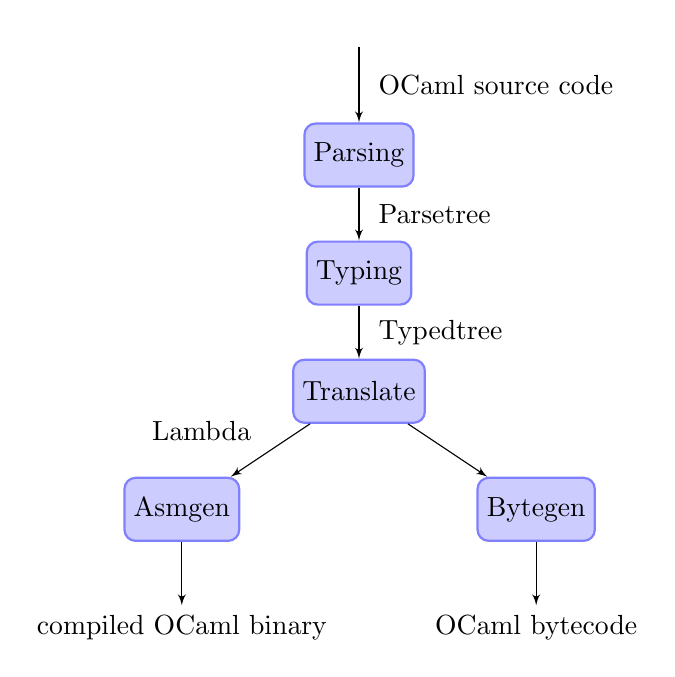
\begin{tikzpicture}[
blank/.style={node distance=1.5cm},
block/.style={rectangle, text centered, rounded corners, minimum height=0.8cm, 
node distance=1.5cm, thick, draw=blue!50, fill=blue!20},
block-emph/.style={block, draw=red!50, fill=red!20},
block-neutral/.style={block, draw=black!50, fill=black!20},
line/.style={draw, -latex'}
]
\node [blank] (start) {};
\node [block, below of=start] (parsing) {Parsing};
\node [block, below of=parsing] (typing) {Typing};
\node [block, below of=typing] (translate) {Translate};
\node [block, below of=translate, xshift=2.25cm] (bytegen) {Bytegen};
\node [blank, below of=bytegen] (compiled-byte) {OCaml bytecode};
\node [block, below of=translate, xshift=-2.25cm] (asmgen) {Asmgen};
\node [blank, below of=asmgen] (compiled-asm) {compiled OCaml binary};

\path [line] (start) -- node [midway, label=right:{OCaml source code}] {}
(parsing);
\path [line] (parsing) -- node [label=right:{Parsetree}] {} (typing);
\path [line] (typing) -- node [label=right:{Typedtree}] {} (translate);
\path [line] (translate) -- node [label=left:{Lambda}, yshift=0.25cm] {} (asmgen);
\path [line] (asmgen) -- (compiled-asm);
\path [line] (translate) -- (bytegen);
\path [line] (bytegen) -- (compiled-byte);
\end{tikzpicture}
    \caption{A representation of the various stages in the OCaml compiler. 
    Adapted from \cite[Chapter~22]{realworldocaml}.}
\end{figure}

The rest of this section will address why this was chosen as the starting 
point, and the process during the preparation phase in which the appropriate 
starting point was determined.

\subsection{Intermediate representations}

The OCaml compiler processes code in the pipeline shown in figure 
\ref{fig:compilerstages}, with the pipeline branching towards the end into two 
separate stages representing the targets that the OCaml compiler can compile 
to. Between each stage, a different intermediate representation of the code is 
produced.

One of the tasks that had to be carried out during the preparation phase was 
to determine which intermediate representation would be most suitable for 
compilation into C. The requirements required for such an intermediate 
representation would be:

\begin{itemize}
\item It must be easy to recover type information from the representation. This 
is because the resulting C code must be statically typed also, so we need to be 
able to infer the types of variables and functions in order for them to be 
implemented in C.
\item The representation must be fairly normalised, with as few as possible 
language constructs to simplify the translation into C. Many language features 
in OCaml are merely syntactically sugared versions of more primitive ones (for 
example, pattern matching is really a combination of branching based on the 
value of a variable plus some variable bindings for unpacking) which must have 
been desugared anyway during the compilation process, so it would be more 
useful if we could utilise an intermediate representation for which this has 
already happened.
\end{itemize}

\subsubsection{\texttt{Parsetree}}

\texttt{Parsetree} is a parsed AST representation of the source code, which 
essentially directly represents the original OCaml source code. No processing 
has occurred on any language constructs, and type inference has not even 
occurred on the IR. This obviously makes this intermediate representation 
unsuitable as the choice of IR, since it falls down on both ability to recover 
type information and normalisation.

\subsubsection{\texttt{Typedtree}}

\texttt{Typedtree} is a type-annotated AST which is almost exactly identical to 
the \texttt{Parsetree} IR, except that expressions have been annotated with a 
type. This makes this IR highly desirable as the starting point for compilation 
into C, and was initially where the investigation for a usable intermediate 
representation started.

However, since \texttt{Typedtree} still almost directly represents the original 
source code, it suffers from the same normalisation problem as 
\texttt{Parsetree} does. For example, the number of different sub-expression 
types that \texttt{Parsetree} represents separately is 31 --- modules, classes 
and objects are still represented as syntactical elements; records, variants, 
and field accesses have not been normalised into one representation; and 
pattern matches have not been simplified but instead stored as association 
lists of raw patterns to expressions.

This makes the \texttt{Typedtree} IR very cumbersome to work with, and 
ultimately it was considered unsuitable for the starting point of the project.

\subsection{The \texttt{Lambda} IR}

The \texttt{Lambda} IR is so named because it resembles an untyped lambda 
calculus, and is what in fact the two existing backends of the compiler 
generate code from. It has a number of advantages over \texttt{Parsetree} and 
\texttt{Typedtree}, including:

\begin{itemize}
\item Variants and records have been normalised into one representation, which 
is referred to as a block, which are similar to tagged unions. In addition, 
variants without parameters are compiled into bare integers.
\item Desugaring of pattern match statements. Because variants have been 
compiled into integers or tagged unions, the translation pass is able to 
optimise pattern matching into switch statements. In very simple cases, pattern 
matches are in fact compiled into an if-else statement instead.
\item Removal of modules and functors. These values have instead been compiled 
into equivalent representations using blocks and functions.
\end{itemize}

In comparison to \texttt{Typedtree}'s 31 different cases for sub-expressions, 
the \texttt{Lambda} representation has 20 different cases, which are relatively 
much simpler than those in \texttt{Typedtree}. This makes the \texttt{Lambda} 
IR far more desirable as a starting point.

However, there are some major disadvantages of the \texttt{Lambda} IR:

\begin{itemize}
\item The translation pass into \texttt{Lambda} does not preserve type 
information from \texttt{Typedtree}. This is a huge problem which is solved 
somewhat with the existence of \texttt{Lambda} events, which will be discussed 
in section \ref{lambda-types}.
\item The \texttt{Lambda} has not yet had closure conversion applied to it. 
Functions are still represented in a similar fashion to how they were in the 
original source code, meaning the cases of lexical closures, partial 
application, etc. are not handled.
\end{itemize}

It was determined that while the \texttt{Lambda} IR does not fully satisfy the 
typing requirement, enough type information was recoverable that it was deemed 
acceptable as a starting point. Thus, my project starts compilation by 
obtaining the \texttt{Lambda} representation by passing the source code through 
part of the compilation pipeline, and then translates the resulting IR into C 
from that point onwards.

\section{Extensibility of GDB}

Part of the project requirements dictate that the resulting code be 
``observable'', and it was quickly identified that if GDB is to be used as the 
primary debugger it may be necessary to extend GDB in order to handle the 
compiled OCaml code correctly and display recursive OCaml values. Thus, a brief 
investigation into GDB was carried out in the preparation phase to investigate 
its extensibility.

One of the experiments which was carried out was to see if GDB could display 
code from other files, and associate parts of compiled C code with instead 
parts of code from another file. This is a necessary part of the compilation 
process, as the resulting debuggable executable must display code and symbols 
from the original OCaml file from which it was compiled from via my compiler, 
not the C file that my compiler produces. With some investigation it was found 
that this was possible with the \texttt{\#}\texttt{line} directive, which will 
be further explored in section \ref{line-directive}.

Another feature which is required for observability is the ability to display 
OCaml values at least recursively, if not formatted in the same way as the 
OCaml compiler does. This is because many OCaml values are recursive (for 
example, the list type is a recursive type which refers back to itself as one 
of its parameters) so it must be possible to extend GDB with some way to 
recursively print values whenever it finds a pointer. It was found that GDB 
does support extensions to itself via custom macros, and also supports custom 
pretty-printers (via, for example, Python) for different types. Either of these 
features would allow GDB to display OCaml values correctly.

\section{Target subsets}

During the write-up of the project proposal, three expanding subsets of OCaml 
were identified in order to structure the creation of the compiler around. 
These subsets represent a grouping of similar constructs and features together 
such that each subset focuses on a similar theme in the new features it 
introduces.

Identification of these subsets firstly has the benefit of providing a clear 
structure to the project, and greatly influenced the order in which features 
were implemented. Optimistically, it was expected that at the end of proposed 
deadlines a compiler would be completed that could compile the associated 
Subset -- unfortunately, due to interdependence between a lot of the features a 
working compiler was not produced until towards the end of implementing 
features for Subset 2.

These subsets also serve to identify what the minimum viable product of the 
project is, as it was determined on project conception compilation of the 
entire OCaml language would be far too ambitious. As such, Subset 3 represents 
the subset of the language that the final product should at minimum be able to 
compile correctly.

Despite the fact that the subsets ultimately did not produce distinct and 
recognisable milestones for compilers that could operate on the appropriate 
subsets of the language, it is still worth describing the subsets for the 
effect they had on the planning for the rest of the project.

\subsection{Subset 1}

Subset 1 is a very simple language with only a limited number of types and 
language constructs. This subset contains only basic boolean, integer, floating 
point, and \texttt{unit} types, only basic string support (for input/output), 
top level function declarations with \texttt{let} and \texttt{let rec}, and 
basic language constructs such as \texttt{if}, \texttt{for}, and \texttt{while}.

The key choices made in this subset were with restricting the amount of 
possible functions and data types greatly. Function definitions could only be 
made at top-level, which means that there was no need to deal with lexical 
closures; in addition, they could only take one parameter so as to sidestep the 
issue with partial application. (This requirement was relaxed as it was found 
to be quite easy to simply restrict function applications to be full 
applications only.)

Otherwise, all data types and language constructs were chosen so that they more 
or less had direct analogues in C code (with the exception of the \texttt{unit} 
type, which was deemed necessary as it was required for imperative-style code 
in OCaml). This in theory made actual implementation details of the compiler 
simple and so the beginning of the project could more be focused on 
demonstrating a working environment and setup.

\subsection{Subset 2}

Subset 2 expands on Subset 1 by introducing custom types and polymorphism. This 
includes tuples, lists, variant types via algebraic data types, record types, 
match expressions and function parametric polymorphism. This subset is aimed 
towards designing and implementing an appropriate representation of OCaml 
values in C, as well as a way of representing polymorphic values both as values 
in user-defined types and as parameters to functions.

The implementation of an OCaml value representation is intended to be a rather 
large milestone, as it would greatly increase the expressiveness of the 
compilable language. Custom user-defined types would allow for implementations 
of custom data structures such as lists, binary trees, etc.

In addition, parametric polymorphism is a large step in terms of 
expressiveness, but its implementation would require some representation of 
polymorphic types and values, which can resolve to a specific type at runtime.

\subsection{Subset 3}

Subset 3 expands further on Subset 2 by adding treatment of functions as first 
class values, plus closure conversion features, which would entail compilation 
of lexical closures, partial application, anonymous functions, etc. The focus 
of this subset is intended towards the design and implementation of closures in 
C, and correctly compiling more difficult parts of OCaml functions into C.

The implementation of this would also allow the representation of higher-order 
functions, such as standard list processing functions \texttt{map} and 
\texttt{filter}, and its completion would indicate the implementation of all of 
the most commonly used features expected to be in a functional language. 

\section{The \texttt{liballocs} library}

A library suggested to me by my supervisor (who happens to be the project 
originator and also the author of the library) is \texttt{liballocs} 
\cite{liballocs}, which is a library that is able to track all allocations in 
memory and their associated types with no extra required effort. It exposes an 
interface that, when given an arbitrary pointer, is able to return information 
about the type of the value in the allocated memory. This was identified to be 
extremely useful for implementing observability features, as it could be used 
within polymorphic functions to determine the type of certain values whilst 
debugging at runtime, which would be an advantage over the OCaml bytecode 
debugger, which due to the untagged nature of OCaml values cannot determine the 
type of polymorphic values at runtime.

\section{Licensing of external code}

As my project only operates on open-source code, software licensing issues are 
not of a great concern to the development of this project. A discussion of the 
licenses in question is included below, however.

The principal body of code being used is the OCaml core system 
\cite{ocamlcompiler}, which is released under LGPL v2.1. LGPL is a more 
permissive version of the GPL license, intended for use for libraries rather 
than full pieces of software. \textbf{TODO -- license discussion}
% TODO - bleh

\textbf{TODO -- Inclusion of the Boehm GC in project}
% TODO

\textbf{TODO -- Use of git to manage source code}

\chapter{Implementation}

In the implementation, several modules were written in OCaml 
for implementing different parts of the compiler. The most significant modules 
were:

\begin{itemize}
\item \texttt{Typecollect}, for obtaining types from the \texttt{Lambda} IR;
\item \texttt{Ccode}, for representation of C compilation target;
\item \texttt{Ccompile}, for the actual compilation process from the 
\texttt{Lambda} IR to C.
\end{itemize}

\section{Obtaining types from the \texttt{Lambda} IR} \label{lambda-types}

A problem encountered early into the project was the fact that the chosen 
intermediate representation, \texttt{Lambda}, did not have any type information 
associated with it. As \texttt{Lambda} was intended as the last representation 
before compilation into actual machine code, all type information was erased 
from the underlying data.

This is a problem for the project. While not having types isn't such a big 
problem for the compilation into C, one of the goals of the project was to have 
the resulting code be ``observable'', which means where possible variables 
should be of the correct type in order for the value to be displayed correctly 
in GDB.

Originally, the \texttt{Typecollect} module attempted to obtain types from the 
\texttt{Typedtree} representation of the code before the transformation into 
\texttt{Lambda}, but it was found that \texttt{Typedtree} expressions do not 
correspond exactly with \texttt{Lambda} expressions. Eventually, a solution was 
found using \texttt{Lambda} events.

\subsection{\texttt{Lambda} Events} \label{levents}

In order for the OCaml compiler to produce debuggable bytecode executables, 
some type information must be passed through the \texttt{Lambda} IR to the 
\texttt{Bytegen} module, as the debugger has to know what type certain 
variables are. It was found that by turning on the debug flag in the compiler, 
it would insert so-called \texttt{Lambda} events into the compiled bytecode.

A \texttt{Lambda} event is simply a wrapper around another \texttt{Lambda} 
expression that carries some extra information. They are defined within the 
OCaml compiler as shown in figure \ref{fig:levent}.

\begin{figure}
    \label{fig:levent}
    \lstinputlisting[language=Caml]{figs/levent.ml}
    \caption{Definition of the \texttt{Lambda} event in the OCaml compiler 
    source code. The \texttt{lambda\char`_event} type stores the attached 
    metadata associated with the event. Of particular note is the 
    \texttt{lev\char`_loc} field, which stores the current source file name, 
    line number and column number corresponding to where this event was 
    inserted, and the \texttt{lev\char`_kind} field, which potentially stores 
    information about the type of the current expression.}
\end{figure}

Within the compiler, the purpose of a \texttt{Lambda} event is to mark where an 
interesting expression may be, in order so that the debugger may stop execution 
and inspect the state of the program just before the evaluation of the 
expression, or just after. In fact \texttt{ocamldebug} does not step between 
lines of code at all -- it steps between \texttt{Lambda} events.

This gives \texttt{Lambda} events two principal useful properties, which are:

\begin{itemize}
\item \texttt{Lambda} events provide information about the current source code 
location of the expressions being currently compiled, which will be useful in 
\ref{line-directive};
\item \texttt{Lambda} events provide type information about types of certain 
expressions.
\end{itemize}

It turns out this is a bit more finicky than one might expect. The compiler 
does not insert events that give types for every expression, nor is there a 
one-to-one correspondence between \texttt{Lambda} expressions and source-code 
expressions, since the \texttt{Lambda} IR may simplify certain expressions or 
insert new ones.

A more reliable approach was found, where it was found that every source-code 
variable was associated with at least one \texttt{Lambda} event describing its 
type; therefore an approach was adopted where the types of variables were 
obtained, and the types of compound expressions were determined with some very 
basic type-inference.

\subsection{The \texttt{Typecollect} module}

Putting this all together, the \texttt{Typecollect} module has a function 
\texttt{scrape} which performs this sequence of instructions:
\begin{enumerate}
    \item Initialise a hash table of variable identifier to types
    (this is safe as the \texttt{Lambda} IR already assigns a different 
    identifier to every variable)
    \item Walk recursively down the \texttt{Lambda} tree:
    {\setlength{\itemindent}{25pt} \item Upon encountering a \texttt{Lambda} 
    event surrounding a variable:}
    {\setlength{\itemindent}{50pt} \item Set the variable and its type in the 
    hash table}
    \item Return the now-filled hash table
\end{enumerate}

The compilation pipeline therefore runs this preliminary pass over the 
\texttt{Lambda} IR before compilation, and then passes the returned types to 
the \texttt{Ccompile} module to inform its compilation process.

\section{Representation of C AST}

Before compilation can start, an appropriate representation of C must be chosen 
as the compilation target for the compiler.

\subsection{Expressions to statements} \label{expr-stmt}

Another of the problems associated with the translation of OCaml into C was the 
fact that the two language had a large difference in syntax. OCaml is what is 
known as an expression-oriented programming language, where every syntactical 
construct is actually an expression of some kind. This is in contrast to C, 
which is statement-oriented -- while expressions exist in C, a block of code in 
C is instead a list of statements, certain constructs can only be written as 
statements (e.g. \texttt{return}, variable declarations), and other constructs 
such as if/while/for statements etc. cannot be used as expressions.

The scheme that my compiler uses to solve this problem is a simple one: every 
sub-expression in the program is assigned to a separate variable. This means 
that if an expression consists of just a variable, use the variable name 
directly; otherwise, create and assign the result of each sub-expression to a 
new temporary variable.

This scheme simplifies the compilation strategy greatly. By setting up a 
variable for each sub-expression, this creates an equivalence between variables 
and sub-expressions. This means that the compilation function need only 
recursively traverse down the \texttt{Lambda} IR tree, adding statements to the 
current context as needed and returning the variable representing the 
expression it was asked to compile. Thus, each sub-expression compiles to a 
block of C statements, at the end of which there is an assignment to a variable 
that holds the value of the expression.

This scheme obviously produces a very large quantity of temporary variables, 
but C compilers have gone through decades of optimisation and often produce 
lots of temporary variables anyway in code transformations such as SSA, so are 
perfectly fine with compiling and optimising code containing large amounts of 
temporary variables. In fact, through my compiler OCaml code without references 
compiles (almost!) into SSA form.

\subsection{The \texttt{Ccode} module}

The \texttt{Ccode} module is an auxiliary module of the compiler that simply 
stores the type declarations for the C AST. This module is not sufficient to 
represent the entirety of the C language, but instead is chosen to represent 
the specific subset of C to which the compiler will target. There are four main 
datatypes in the module, and a quick summary of them is given here:

\begin{enumerate}
\item \texttt{Ccode.cident}, for representing identifiers (variable names, 
macro names, function names etc.) in C. This is largely a wrapper over the 
\texttt{Ident.t} type the OCaml compiler uses to represent identifiers, which 
is the string name along with a unique integer ID to disambiguate it from other 
identifiers with the same name.

\item \texttt{Ccode.cexpr}, for representing expressions in C. These include a 
wrapper around \texttt{cident}s, literals, and operations (such as unary 
operations, binary operations, function calls etc.) on other 
\texttt{cexpr}s.

\item \texttt{Ccode.cstatement}, for representing statements in C. Most data 
constructors in this type take a \texttt{cexpr} or a block of other 
\texttt{cstatement}s, and include if statements, while statements, switch 
statements etc. Notably a \texttt{cexpr} can be promoted to a 
\texttt{cstatement}, but not the other way around.

\item \texttt{Ccode.ctype}, for representing types in C. This is a auxiliary 
type used by the casting operator in \texttt{cexpr} and the variable 
declaration statement in \texttt{cstatement}. A more in-depth discussion of the 
types used to represent OCaml values is at section \ref{value-repr}.

\end{enumerate}

\subsection{The \texttt{Cprint} module}

The \texttt{Cprint} module is another module that's fairly straight-forward -- 
it contains functions for printing types from \texttt{Ccode} to an output 
stream, most likely a file. There's not anything very complicated going on in 
this module -- the functions simply recursively traverse down the C ``AST'' and 
prints out the corresponding C as it goes along.

\subsection{\texttt{\#}\texttt{line} directives} \label{line-directive}

One feature to do with observability which would be prudent to discuss here is 
use of the so-called \texttt{\#}\texttt{line} directive. A key observability 
feature is for the debug table to associate sections of the output code with 
the relevant line from which they were compiled from, which allows debuggers 
such as GDB to display to the user a listing of the relevant source code, and 
associate the currently executing machine code with the correct line of source 
code.

Naturally this ability is highly desirable for this compiler. Luckily, the C 
preprocessor supports controlling the line and source file of your code with 
use of the \texttt{\#}\texttt{line} directive, by inserting it in the source 
code in the format \verb|#line linenum filename|. This provides a compilation 
strategy for the compiler, which to compile all statements as being on the same 
line (the line number changes whenever there is a new line, even after being 
specified with \verb|#line|), interspersed with a \verb|#line| directive 
whenever the source code line actually changes.

One final question is, where do we obtain information about which line a 
\texttt{Lambda} expression is from? \texttt{Lambda} expressions typically do 
not map to source-code expressions, nor do they contain information about which 
line the expression originates from. This is the second place where 
\texttt{Lambda} events are useful (refer back to \ref{levents}) -- they carry 
information about the current file and line. Also, since they represent places 
where the OCaml bytecode debugger \texttt{ocamldebug} may pause execution, this 
gives us a pleasing way to treat them: \texttt{Lambda} events compile into 
\verb|#line| directives.

\section{Compilation of basic constructs}

After the initial foundations of the compiler were made, structures from Subset 
1 in the proposal were implemented first. These encompass simple structures 
which have similar analogues to structures in C.

\subsection{Variable scoping differences between C and OCaml} 
\label{variable-scoping}

Before diving into the implementation of these expressions, one issue that 
needs to be addressed is the differences in variable scoping between the two 
languages. This is a significant detail when considering observability -- we 
would like the debugger to print out the contents of the correct variable 
within a scope when prompted.

In OCaml, each variable is only visible in the body of the expression where it 
is bound, whether if that's in a let-binding or a function declaration. This is 
in contrast to variable scope in C, where a variable is visible for the 
entirety of the rest of the block it is in.

Furthermore, while OCaml does not allow reassignments (of variables, not 
references), it does allow you to bind another variable with the same name, 
which you can see in the short snippet:

\begin{lstlisting}[language=Caml]
let x = 1 in
let x = 2 in
print_int x
\end{lstlisting} 

Here the second binding is not reassigning the value of \texttt{x}, rather it's 
creating another variable with the same name. The first variable still exists, 
but it's been shadowed by the second variable making it inaccessible. Note that 
after leaving the body of the second let binding the second variable goes out 
of scope and the first variable is accessible again.

This behaviour can be approximated using block-scoping in C, since variable 
scopes are limited to the block they were created in C and local variables 
shadow variables in an outer scope. It's worth noting that however, this does 
not work for file-level variables, since you cannot create blocks of code at 
the file-level -- all file-level variables must live in the same scope.

\subsection{\texttt{let} bindings}

With the differences in variable scoping between C and OCaml appreciated, 
particular care has to be taken when compiling a \texttt{let} binding. In 
OCaml, a \texttt{let} binding has the structure:

\begin{center}
    \texttt{let \emph{x} = \emph{expr} in \emph{body}}
\end{center}

Note that \texttt{\emph{x}} is not a free variable of \texttt{\emph{expr}} 
but is one in \texttt{\emph{body}}, and also that the value of the overall 
expression is the evaluated value of \texttt{\emph{body}}. Thus, a block is 
required to emulate the scoping correctly.

The resulting structure that a \texttt{let} binding compiles into is shown 
therefore by this C-style pseudocode. Recall that according to the compilation 
strategy outlined in section \ref{expr-stmt}, each OCaml expression compiles to 
a block of C statements, at the end of which the value of the expression is 
assigned to a variable. We will therefore adopt the notation where for an OCaml 
expression \texttt{X}, \texttt{comp[X]} denotes the block of C statements 
\texttt{X} compiles into, and \texttt{var[X]} denotes the C variable that the 
value of \texttt{X} is assigned to.

\begin{lstlisting}
decl result;

comp[expr];
decl temp = var[expr];
{
    decl x;
    x = temp;
    
    comp[body];
    result = var[body];
}
\end{lstlisting}

Things of note here is that \texttt{\emph{expr}} must be evaluated outside of 
the inner scope, where \texttt{\emph{x}} is visible, and \texttt{\emph{body}} 
must be evaluated inside the inner scope. We declare and assign the value of 
\texttt{\emph{x}} only inside the inner scope. In addition, the actual value of 
\texttt{\emph{expr}} must then be available outside the inner scope, so we 
propagate it outwards by declaring a variable \texttt{result} in the outer 
scope and performing its actual assignment in the inner scope.

The other detail is that OCaml allows \texttt{let} bindings to be a shorthand 
for function declaration; function compilation will be discussed in section 
\ref{functions}.

\subsection{\texttt{if-then-else} expressions}

OCaml does not have if-statements but if-expressions, which are of the form:

\begin{center}
    \texttt{if \emph{cond} then \emph{A} else \emph{B}}
\end{center}

Using the same notational conventions as the previous section, this compiles 
into the pseudocode:

\begin{lstlisting}
decl result;

comp[cond];
if (var[cond]) {
    comp[A];
    result = var[A];
}
else {
    comp[B];
    result = var[B];
}
\end{lstlisting}

The same trick to propagate results outwards from inner scopes has been 
employed here also.

\subsection{\texttt{while} loops}

While loops are fairly simple in OCaml -- they simply repeatedly evaluate their 
body while the condition evaluates to true. There are no break nor continue 
statements, so there is not a concept of breaking out of a loop early with the 
exception of setting the condition to false. They have the syntax:

\begin{center}
    \texttt{while \emph{cond} do \emph{body} done}
\end{center}

In addition, the overall return value of the loop is \texttt{unit}. This 
therefore translates into the following pseudocode:

\begin{lstlisting}
comp[cond];
while (var[cond]) {
    comp[body];
    comp[cond];
}

decl result = make_unit();
\end{lstlisting}

There is one interesting thing of note here: \texttt{\emph{cond}} does need to 
be evaluated twice, once before the loop, and once at the end of the loop. This 
is because the OCaml while loop re-evaluates \texttt{\emph{cond}} at the 
beginning of each iteration, but since OCaml expressions turn into a list of 
statements in C, we cannot fit this re-evaluation into the head of the while 
statement -- instead, a simple and equivalent way around this is to simply 
re-evaluate \texttt{\emph{cond}} at the end of the loop.

A discussion of the way the \texttt{unit} type is implemented will be in 
section \ref{value-repr}.

\subsection{\texttt{for} loops}

For loops in OCaml are extremely limited. They permit only iteration over a 
fixed range of integers, and also only allow increments in steps of 1. Like 
with while loops, there are no break nor continue statements in OCaml and so 
there is no possibility of exiting a loop early. They have two forms, which are:

\begin{center}
\texttt{for \emph{x} = \emph{start} to \emph{end} do \emph{body} done}\\
\texttt{for \emph{x} = \emph{start} downto \emph{end} do \emph{body} done}\\
\end{center}

These two versions simply iterate up to or down to a certain number 
(inclusive). Since for loops are so incredibly limited, it was decided 
that rather than including for loops in the targeted subset of C, it would be 
easier to also compile these into while loops in C.

\begin{lstlisting}
comp[start];
comp[end];
int temp1 = var[start];
int temp2 = var[end];

{
    decl x = temp1;
    while (x <= temp2) {
        comp[body];
        x++;
    }
}

decl result = make_unit();
\end{lstlisting}

(Replace \texttt{<=} for \texttt{>=} and \texttt{x++} for \texttt{x--} for 
\texttt{downto}.)

There are a few things about this compilation that warrant elaboration:
\begin{itemize}
\item \texttt{\emph{x}} again needs to be declared in its own scope, as the for 
loop acts as another variable binding site. Thus, the entirety of the for loop 
is wrapped in another block.

\item Note the use of \texttt{temp1} and \texttt{temp2}, which are necessary 
because \texttt{var[start]} and \texttt{var[end]} may collide with the name of 
the variable \texttt{x} and cause it to be shadowed in the inner scope.

\item \texttt{\emph{start}} and \texttt{\emph{end}} are only evaluated once at 
the start of the loop -- after some quick experiments it could be shown that 
OCaml does this as well, i.e. the limits of the iteration range do not change 
while the loop is running.

\item \texttt{\emph{x}} is mutated through the iteration of the loop. This is 
fine, as OCaml for loops only operate on integers, which are copied instead of 
referenced by other constructs in the target subset of C; thus the mutation of 
\texttt{\emph{x}} cannot affect the behaviour of the program.
\end{itemize}

\subsection{Recursive bindings with \texttt{let rec}}

Normally in a let binding, the variable being bound is not in scope for the 
expression being bound. This however makes it difficult to define recursive 
functions, so OCaml supplies the \texttt{let rec} binding which is useful for 
creating recursive of sets of mutually recursive functions.

However OCaml allows \texttt{let rec} bindings to be used for creating a 
restricted class of non-functional recursive values. The typical example given 
(as adapted from the OCaml manual) is:

\begin{center}
    \texttt{let rec x = 1::y and y = 1::x in \emph{expr}}
\end{center}

This binds \texttt{x} to the infinite list \texttt{1::2::1::2::...}, which is 
accomplished by making the list cyclical -- that is, it points back it itself.

Informally, the class of values that are allowed to be used as the right-hand 
side of a \texttt{let rec} binding are those where the recursively bound names 
occur only within a function, or a data constructor. This means that to 
preserve the semantics in C, the variables should be first initialised with 
\texttt{malloc} to determine their pointers. Once the pointers are determined, 
compilation proceeds as normal using the newly-determined pointers when 
referring to the variable.

The compiler thus splits compilation of \texttt{let rec} into two phases:

\begin{itemize}
    \item Firstly, variables are declared. If the associated expression has no 
    free variables, compilation can happen straight away; otherwise, the size 
    of the resulting value in memory is determined and a pointer is obtained 
    using \texttt{malloc}.
    
    \item Once all the pointers are known, compilation proceeds as normal with 
    assignments going to the declared variable name instead of a locally 
    created variable.
\end{itemize}

\section{OCaml value representation} \label{value-repr}

An important aspect of the compiler is the design of the representation of 
OCaml values within C. OCaml has a rather different data-type model to C, so an 
appropriate design of value representations is not only crucial to the 
correctness and speed of the compiler, but also to the observability of the 
resulting code.

An example of this is that the OCaml compiler discards type information in its 
compilation process, so that the type information at runtime cannot always be 
determined. This is detrimental to the observability of its debugger, as 
\texttt{ocamldebug} for example cannot determine the actual types of 
polymorphic values at runtime and so cannot display their values, opting only 
to display \texttt{<poly>}.

This section largely details work undertaken to implement Subset 2, which deals 
with data representation and the language structures surrounding them.

\subsection{Representation requirements}

Before discussing the strategy for representing OCaml values, it is useful to 
explore the exact problems that the value representation are aiming to solve, 
which will in turn motivate its design.

\subsubsection{Basic types}

OCaml has a number of primitive types, which have analogues in C. These can be 
translated directly in most cases. These include \texttt{int}, \texttt{float}, 
\texttt{bool}, \texttt{string}, and \texttt{char}.

\subsubsection{Integer types}

Simple values and variants are represented as integers within OCaml. For 
example, the \texttt{unit} type is represented with the OCaml integer 0, and 
variants with no parameters are represented as integers, e.g. in \texttt{type 
test = Foo | Bar}, \texttt{Foo} is represented by the integer 0 and 
\texttt{Bar} by the integer 1.

\subsubsection{OCaml blocks}

More complex types such as variants with parameters, tuples, and records are 
represented by a construct known as an OCaml block, which is a variable length 
array of values with a header containing its length and an integer tag, which 
is used to differentiate between different variants and types of blocks. An 
example is \texttt{type test = A of int | B of float | C of str} -- \texttt{A} 
will construct a block containing an \texttt{int} with tag 0, \texttt{B} will 
construct a block containing a \texttt{float} with tag 1, and \texttt{C} will 
construct a block containing a \texttt{str} with tag 2.

The \texttt{Lambda} IR in fact normalises all data structures into blocks, 
including references (they're a mutable singleton block), arrays, modules etc. 
which is rather convenient as we can implement all of these data types for free 
by implementing blocks.

\begin{figure}
    \label{fig:block-header}
    \centering
    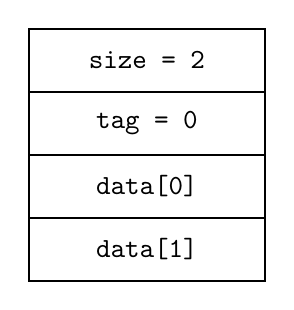
\begin{tikzpicture}[
blank/.style={node distance=0.8cm, font=\ttfamily},
block/.style={rectangle, text centered, thick, draw=black, font=\ttfamily,
    minimum width=3cm, minimum height=0.8cm, node distance=0.8cm},
block-header/.style={block, node distance=5cm},
block-body/.style={block},
line/.style={draw, thick, *-latex', shorten <=-1.2mm}
]

\node [block-header] (size) {size = 2};
\node [block-body, below of=size] (tag) {tag = 0};
\node [block-body, below of=tag] (data-0) {data[0]};
\node [block-body, below of=data-0] (data-1) {data[1]};
\end{tikzpicture}
    \caption{Example OCaml block containing two values with tag 0, with a 
    header containing the current size and tag of the block, followed by the 
    values of the block.}
\end{figure}

\subsubsection{Polymorphic types}

Code in polymorphic functions may not know the type of variables they're 
manipulating, so cannot deal with variably-sized data as they may not copy or 
pass polymorphic values correctly.

\subsection{Representation strategy}

As a basic consequence of the fact that we want the resulting C code to be 
observable, whenever there is a basic type the C code should endeavour to use 
the equivalent type in C as much as possible. Thus for simple cases the 
translation and representation is straightforward -- simply replace the OCaml 
type with the corresponding C type.

Representation for non-primitive types however is more complex. Integer types 
and OCaml blocks must be unified somewhat in representation, because variants 
that don't have any parameters and variants that do can be of the same type; 
for example, in \texttt{type test = Foo | Bar of string}, \texttt{Foo} is 
represented by the integer 0, but \texttt{Bar} is represented by an OCaml block 
with tag 0 and the string as its first element, but these need to be 
represented as the same type despite one being variably-sized.

\subsubsection{Tagged pointers}

The solution to this therefore is to employ a tagged pointer structure. 
Firstly, OCaml blocks must be allocated on the heap since they are 
variably-sized, so we must reference them using a pointer. This means that we 
need a union type which combines a pointer and an integer, which is what a 
tagged pointer representation does.

Tagged pointers take advantage of the fact that on most architectures, pointers 
are word-aligned. This means that the lower bits of a pointer are always 0, 
which means that it's possible to store extra bits of information in the lower 
bits of a pointer, and just zeroing those bits out when you need to dereference 
the pointer. In the architecture I am developing on, which is 64-bit Linux, 
pointers are always aligned to 8-bytes -- this leaves 3 free bits at the end of 
any pointer.

The tagged pointer approach employed in this compiler is to use the least 
significant bit of an 8-byte word as the tag bit to differentiate between 
pointers and integers. This does mean that integers will lose one bit of 
precision, but in fact the OCaml native runtime uses either 31-bit or 63-bit 
integers as well depending on the architecture.

There is a choice as to which way round the tag bit should be -- should 0 
represent integers or pointers? It was chosen to use 0 for pointers, and 1 for 
integers, which means that the ``boxed'' version of a pointer is identical to 
the pointer in memory. This choice was made on two bases:

\begin{itemize}
    \item Dereferencing pointers is far more common than integer maths (which 
    also happen to representing variants, not actual integers), so no extra 
    work needs to be performed to dereference a boxed pointer.
    \item Since boxed pointers are exactly the same as they were prior to being 
    boxed, this means that it is incredibly easy to use a conservative garbage 
    collector as a drop-in replacement. This is discussed further in section 
    \ref{gc}.
\end{itemize}

It is noted here that an alternative approach to boxing pointers exists and is 
common in implementations of other languages, in particular JavaScript, which 
is NaN-boxing. The concept is to utilise the unused ``NaN-space'' of values in 
IEEE 754 floating point numbers to store integers and pointers, meaning that 
this approach is able to store floating point numbers as immediates as well as 
integers. This approach was not chosen because of the relative complexity of 
implementation, extra reduced precision for integers, and poor interopability 
with existing conservative GC implementations.

\subsubsection{Polymorphic values}

Now that we have one consistent representation for integers and arbitrary 
blocks, which always takes up one word, it's very tempting to use this to 
represent polymorphic values as well. If all values can be represented using a 
word-sized structure, this solves the problem of not knowing what size a 
polymorphic value is.

This is because the only operation that could be performed on a polymorphic 
value is copying it somewhere or passing it as a parameter to another function 
-- if the type was more concretely known at any point, it would've been 
possible to obtain a more concrete type from the \texttt{Lambda} IR.

The solution is therefore to ``box'' all types as the tagged pointer 
representation. Since the pointer part of the tagged pointer representation 
always points to an OCaml block, we create special OCaml blocks for holding 
other primitive types such as floating point numbers and strings. To 
disambiguate these blocks from other normal blocks so that at runtime, the 
debugger is able to see what type they really are, we assign a special tag to 
them which marks the block as containing only floats or strings or etc.

\begin{figure}
    \label{fig:block-example}
    \centering
    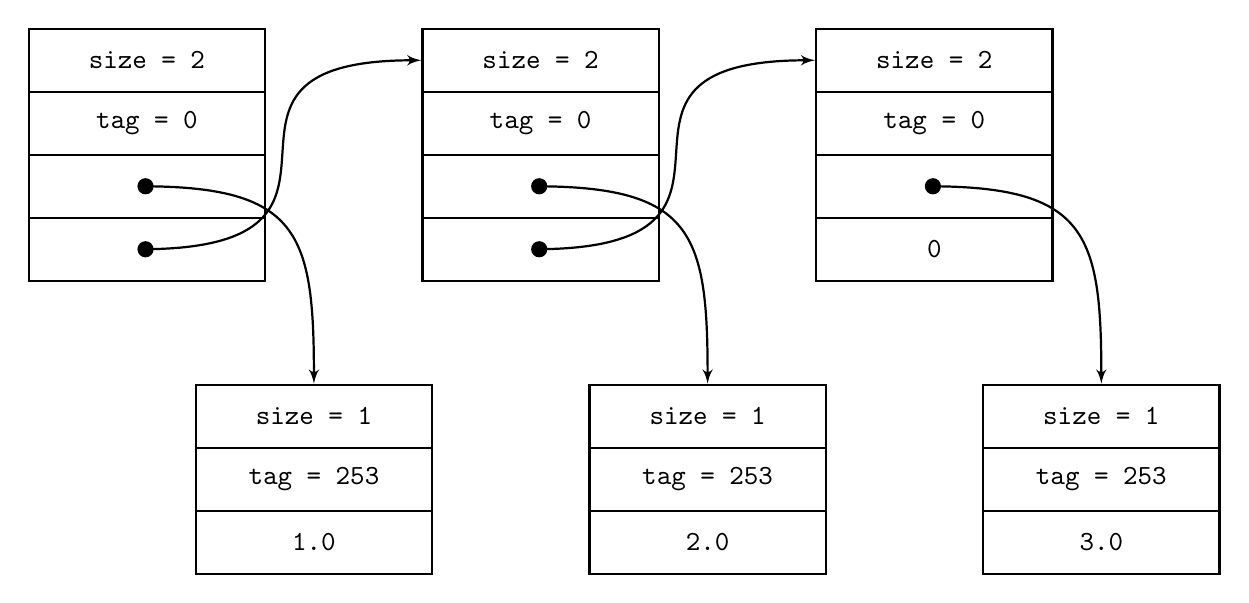
\begin{tikzpicture}[
blank/.style={node distance=0.8cm, font=\ttfamily},
block/.style={rectangle, text centered, thick, draw=black, font=\ttfamily,
    minimum width=3cm, minimum height=0.8cm, node distance=0.8cm},
block-header/.style={block, node distance=5cm},
block-body/.style={block},
line/.style={draw, thick, *-latex', shorten <=-1.2mm}
]

\node [block-header] (a-size) {size = 2};
\node [block-body, below of=a-size] (a-tag) {tag = 0};
\node [block-body, below of=a-tag] (a-data-0) {};
\node [block-body, below of=a-data-0] (a-data-1) {};

\node [block-header, right of=a-size] (b-size) {size = 2};
\node [block-body, below of=b-size] (b-tag) {tag = 0};
\node [block-body, below of=b-tag] (b-data-0) {};
\node [block-body, below of=b-data-0] (b-data-1) {};

\node [block-header, right of=b-size] (c-size) {size = 2};
\node [block-body, below of=c-size] (c-tag) {tag = 0};
\node [block-body, below of=c-tag] (c-data-0) {};
\node [block-body, below of=c-data-0] (c-data-1) {0};

\node [block-header, below right of=a-data-1, node distance=3cm] (d-size) {size 
= 1};
\node [block-body, below of=d-size] (d-tag) {tag = 253};
\node [block-body, below of=d-tag] (d-data-0) {1.0};

\node [block-header, below right of=b-data-1, node distance=3cm] (e-size) {size 
= 1};
\node [block-body, below of=e-size] (e-tag) {tag = 253};
\node [block-body, below of=e-tag] (e-data-0) {2.0};

\node [block-header, below right of=c-data-1, node distance=3cm] (f-size) {size 
= 1};
\node [block-body, below of=f-size] (f-tag) {tag = 253};
\node [block-body, below of=f-tag] (f-data-0) {3.0};

\path [line] (a-data-0.center) to [out=0, in=90, looseness=1.5] (d-size);
\path [line] (a-data-1.center) to [out=0, in=180, looseness=2] (b-size);

\path [line] (b-data-0.center) to [out=0, in=90, looseness=1.5] (e-size);
\path [line] (b-data-1.center) to [out=0, in=180, looseness=2] (c-size);

\path [line] (c-data-0.center) to [out=0, in=90, looseness=1.5] (f-size);

\end{tikzpicture}
    \caption{Example box-and-pointer diagram for the list \texttt{[1.0; 2.0; 
    3.0]}. As lists are linked lists in OCaml, each node in the list contains 
    the OCaml value of its element, and the next value in the list, which is 
    either a pointer to the next node or the OCaml value \texttt{[]}, 
    represented by the integer 0. Floating point numbers must be boxed to be 
    stored in a block, so a new block is created for each one. These blocks 
    have the special tag 253, which indicates that their contents is a floating 
    point number.}
\end{figure}

\subsection{Representation in C} \label{c-repr}

By taking advantage of flexible array members, it is easy to implement an OCaml 
block in C.

\begin{lstlisting}[language=C]
typedef struct _block {
    uintptr_t size : 56;
    uintptr_t tag : 8;
    any_type data[];
} block;
\end{lstlisting}

Recall that a block needs to store its size, an integer tag, and any number of 
other OCaml values. On a standard 64-bit architecture the address space is only 
$2^{48}$ bytes large, and considering that we only need to store words which 
are 8 bytes on 64-bit Linux the maximum that \texttt{size} could be is $2^{45}$.
In addition, OCaml tags only range between 0 to 255\footnote{In fact, the 
native OCaml runtime restricts the number of possible variants to 246, using 
the tags 0-245 for variants. It uses the last 10 possible tags for special 
tags, such as tagging floats, strings, abstract values etc.}. We can therefore 
reduce the amount of space used for the header using C bit-fields, allocating 8 
bits to \texttt{tag} and the remaining 56 bits to \texttt{size}, meaning the 
header is only one word long.

Now we have a block definition, we can implement actual OCaml values as being a 
simple union type:

\begin{lstlisting}[language=C]
typedef union _value_type {
    intptr_t i;
    block* block;
} value_type;

#define BOX_INT(v) ((value_type){.i = (intptr_t)(v) << 1 | 1})
#define UNBOX_INT(v) ((v).i >> 1)

#define BOX_BLOCK ((value_type){.block = (v)})
#define UNBOX_BLOCK ((v).block)

#define IS_INT(v) ((v).i & 1)
\end{lstlisting}

\verb|BOX_INT| and \verb|UNBOX_INT| demonstrate how to box integers into a 
\verb|value_type|, and likewise for block pointers. We also have a special 
macro \verb|IS_INT|, which checks if a \verb|value_type| is holding an integer 
or a pointer -- it simply checks the last bit, returning 1 if the last bit is 
also a 1.

One final thing to talk about is the purpose of \verb|any_type|, which one may 
have noticed in the definition of \verb|block|. Blocks normally hold an array 
of \verb|value_type|s, but there are special blocks which hold strings and 
floating point numbers. This means that blocks actually need to hold a union 
type, which is defined thusly:\footnote{For clarity, we're ignoring the 
problems associated with recursive type definitions in C, and assuming that we 
have the correct forward declarations.}

\begin{lstlisting}[language=C]
typedef union {
    intptr_t i;
    uintptr_t u;
    double fl;
    char* str;
    value_type value;
    closure_type* closure;
    (void*)(*f)();
} any_type;
\end{lstlisting}

We use a union for this kind of type-punning instead of doing a pointer cast 
with a \verb|void| pointer for example to avoid violating the strict aliasing 
rule, which allows the output of our compiler to be optimised more greatly by C 
compilers. Another detail is that the \verb|any_type| union also holds 
integers, function pointers, and closures as it is reused for the closure 
representation, which will be discussed in section \ref{functions}.

\subsection{Type casting} \label{casting}

While the \texttt{Lambda} IR has already gone through type inferencing and thus 
types should have been already determined and statically checked, there are 
still a few cases in which a cast is necessary from one type to another. These 
cases are:

\begin{itemize}
    \item A cast from an integer to an OCaml value is required, because the 
    \texttt{Lambda} IR uses integers for representing certain non-integer OCaml 
    values.
    \item A cast from any type to an OCaml value, because a variable is being 
    passed into a polymorphic function, or being placed into a block.
    \item An actual cast function between types, such as from integers to 
    floating point numbers.
\end{itemize}

A very simple algorithm is used therefore whenever there is a type mismatch 
between two variables in the cases of assignment and passing arguments to 
functions or closures.

\begin{enumerate}
\item If the source and target types are the same, do nothing.
\item If the source type is \verb|any_type|, unpack the union according to the 
target type.
\item If the target type is \verb|any_type|, pack the value into another 
\verb|any_type|.
\item If the source type is \verb|value_type|, unbox the value according to the 
target type.
\item If the target type is \verb|value_type|, box the value into anotehr 
\verb|value_type|.
\item Otherwise, perform a C cast between source type and target type.
\end{enumerate}

\subsection{Pattern matching}

OCaml employs pattern matching in many constructs of the language, particularly 
in its \texttt{match} expressions. Fortunately, the \texttt{Lambda} IR usually 
compiles these down to an equivalent set of \texttt{if} expressions and 
\texttt{let} bindings. In the case of variants however, pattern matching 
typically compiles down into a \texttt{Lambda} expression called the 
\texttt{Lswitch} expression.

\subsubsection{\texttt{Lswitch} expressions}

\texttt{Lswitch} expressions correspond to match statements on a variant 
expression. For an example, consider the type and match expression:

\begin{lstlisting}[language=Caml]
type color =
  | Red
  | Green
  | Blue
  | Gray of int
  | RGB of int * int * int

match c with
  | Red -> 0
  | Green -> 1
  | Blue -> 2
  | Gray x -> 3
  | RGB (r, g, b) -> 4
\end{lstlisting}

In the type \texttt{color}, \texttt{Red}, \texttt{Green} and \texttt{Blue} will 
be compiled into the OCaml integers 0, 1, and 2, and \texttt{Gray} and 
\texttt{RGB} are compiled into blocks with the tags 0 and 1 respectively. This 
match statement is compiled into the following \texttt{Lambda} expression:

\begin{lstlisting}
(switch* c/xxxx
  case int 0: 0
  case int 1: 1
  case int 2: 2
  case tag 0: 3
  case tag 1: 4)
\end{lstlisting}

This looks fairly similar to a switch statement in C, but there's one 
important difference: each the cases predicate on both whether the value is an 
integer or a block and the value of its value/tag.

One \texttt{Lswitch} statement therefore compiles into two switch statements in 
C, one for the integers and one for the tags, which are the two branches of an 
if statement that checks if the value being switched on is an integer or a 
value, using the \verb|IS_INT| macro defined earlier.

\subsubsection{\texttt{Lstaticraise} and \texttt{Lstaticcatch}}

The \texttt{Lambda} IR actually has support for static exceptions, which are 
exceptions that can only occur across a local scope (in contrast to normal 
exceptions, which unwind the stack and can jump to an error handler in an 
enclosing scope). In particular, the OCaml pattern-match compiler may opt to 
use a static exception to avoid duplication of code for certain branches. For 
example, consider this match expression:

\begin{lstlisting}[language=Caml]
match c with
  | Red -> 0
  | Green -> 1
  | Gray x -> 2
  | _ -> 3
\end{lstlisting}

This match expression contains a wildcard expression which matches both 
\texttt{Blue}, which is an integer, and \texttt{RGB}, which is a block. The 
OCaml pattern-match compiler thus compiles it into the following 
\texttt{Lambda} expression:

\begin{lstlisting}
(catch
  (switch* c/xxxx
    case int 0: 0
    case int 1: 1
    case int 2: (exit 1)
    case tag 0: 2
    case tag 1: (exit 1))
  with (1) 3)
\end{lstlisting}

The branches for \texttt{Blue} and \texttt{RGB} have been compiled into a 
static exception, to avoid duplicating the expression in the branch. Luckily in 
C this can be very simply emulated with gotos. \texttt{Lstaticcatch} 
expressions can be compiled simply into an \texttt{if(0)} and a label, and 
\texttt{Lstaticraise} expressions are simply compiled into a goto.

\section{Function compilation and closure conversion} \label{functions}

Functions and closures are the last hurdle to overcome for compiling OCaml into 
C. As OCaml is a functional language, functions have many more features than in 
C, including creating closures, freezing the environment of a function into a 
value.

OCaml has support for first class functions, allowing functions to be used as 
values. C does not have support for this -- it supports a limited form of this 
using function pointers, but this is not sufficient for the representation of 
closures in C. The following sections will discuss the motivations for a 
closure representation and the implementation of such a representation.

\subsection{Local functions}

All functions in C are required to be defined at top-level, which means that 
nested function declarations are not possible. This is in contrast to OCaml, 
where function definitions are simply expressions like any other, and thus can 
be defined locally and passed as values. In order to emulate this behaviour in 
C, whenever we come across a function definition we lift the function 
definition to the toplevel scope, compile the function there, and then return 
its function pointer when we come back.\footnote{This clearly does not deal 
with lexical closures, so we actually return a pointer to a closure object 
instead of a function pointer, but the idea is the same.}

\subsection{Function Typing} \label{function-typing}

In OCaml, one way of thinking about functions is to view them as only ever 
being functions of one argument, which return other functions. As an example, 
the function type \texttt{int -> float -> int} represents a function that takes 
an integer and returns a \texttt{float -> int}, which is a function that takes 
a floating point number and returns an integer. It can be seen that \texttt{->} 
is really a right-associative operator on types; a function type \texttt{'a -> 
'b -> 'c -> 'd} should be bracketed as \texttt{'a -> ('b -> ('c -> 'd))}.

While this is a correct high-level view of functions and explains how partial 
application works nicely, this is not suitable for a low-level implementation 
at all -- it is much more efficient for functions to actually accept multiple 
arguments, instead of returning a succession of other functions for which each 
need to be successively constructed and have the just-applied value saved to 
the environment of the function. In addition, successively calling functions 
increases the amount of stack manipulation that takes place, and not passing 
multiple arguments at once means that the compiler is not able to take 
advantage of optimisations where arguments are passed by registers instead of 
stack-spilling.

In C by contrast, a function declaration consists of a return type, and a list 
of input arguments. We therefore need a consistent conversion between OCaml 
function types and C function types, so we pick the most obvious one -- all the 
types in the OCaml function type are the arguments to the C function, and the 
final type is the return type of the C function. Thus, a function of type 
\texttt{int -> float -> str} is compiled to \texttt{char* (*)(int, double)} in 
C.

\subsubsection{Functions that return other functions} \label{incomplete-funcs}

While functions in OCaml are usually declared as if they take in multiple 
arguments and return a value, it is possible and often useful to define 
functions that return other functions. As a simple example, consider the 
function:

\begin{lstlisting}[language=Caml]
let f x = (fun y -> x + y)
\end{lstlisting}

The type of \texttt{f} is \texttt{int -> int -> int}, but it's obvious that 
this isn't translatable into a C function \texttt{int f(int x, int y)} -- the 
body of the function would return a function pointer, and not an integer.

This is actually a rather simple problem to fix via a technique known as 
eta-expansion, and can be done at the source code level. Simply add extra 
parameters to match the number of parameters in the type, and apply them to the 
old result of the function.

\begin{lstlisting}[language=Caml]
let f x y = (fun y -> x + y) y
\end{lstlisting}

\subsection{Closure representation}

Closures are, implementation-wise, a structure that stores both a function 
pointer and an environment, containing values required for the execution of the 
function.

Our closure representation essentially requires storing a function pointer and 
some list of values, so taking advantage of flexible array members again we 
arrive at the following definition:

\begin{lstlisting}[language=C]
typedef struct _closure_type {
    void* (*f)();
    struct _closure_type* next;
    any_type args[];
}
\end{lstlisting}

As you can see, this definition contains a function pointer, and a 
variably-sized array of arguments, which we reused \verb|any_type| from section 
\ref{c-repr} to implement. One interesting choice taken here is that closures 
also have a \texttt{next} field which points to another \verb|closure_type|, 
allowing them to act like a linked list -- the motivation of this is discussed 
in partial application compilation, in section \ref{partial-app}.

\subsubsection{Promoting functions to closures}

Now that we have a closure object, we need some way for functions to actually 
access the contents of the closures. The way this is implemented is to add an 
extra parameter to the end of the arguments of any closure, 
\verb|closure_type* closure_obj|, which stores the pointer to the current 
closure object. From there, the function is able to access closure values by 
indexing \verb|closure_obj->args|.

This necessitates some sort of promotion process where functions that do not 
require closures are promoted to closures. This is simple to do by creating 
another function which takes all the same arguments as the original function 
plus one more, which is the closure object. This function just passes the 
arguments along to the original function.

\begin{lstlisting}[language=C]
return_type promoted_closure(...args, closure_type* closure_obj) {
    return f(...args);
}

closure_type* cl = MALLOC(sizeof(closure_type));
cl->f = (void*(*)())&promoted_closure;
cl->next = NULL;
\end{lstlisting}

\subsubsection{Calling closures}

Calling a closure can be done by invoking the function pointer with the 
required arguments, passing in the closure pointer as the last argument.

\begin{lstlisting}[language=C]
cl->f(...args, cl);
\end{lstlisting}

As one can see from the previous section, \texttt{cl->f}, which is 
\verb|&promoted_closure|, correctly translates this call into a call of 
\texttt{f} with the correct arguments.

\subsubsection{Unification of closures and functions}

Closures and functions are indistinguishable and practically the same thing in 
OCaml, so for ease of representation, it was decided to unify functions and 
closures in C as well. This means that all functions are promoted to closures, 
and all function applications in OCaml are compiled into closure calls in C.

While this simplifies the implementation, it does come at a large performance 
cost of needing to allocate extra memory whenever new closures are created, as 
well as causing function calls to go through an extra layer of indirection. 
Surprisingly however, experiments have shown that modern C compilers are able 
to successfully detect references to other functions in this representation, 
and even perform tail-call optimisation in spite of this.

\subsection{Partial application compilation} \label{partial-app}

Partial application is one of the major use-cases for closures, whereby 
programmers can create new functions by not passing all required parameters to 
a function. Operationally, this means that the value of the parameter is saved 
in a closure, and once enough arguments have been applied to the closure the 
parameter is passed as the first argument along with the other arguments to the 
original function.

This is modelled using a closure object. Whenever there is a partial 
application, a function is created instead that takes remaining parameters, and 
a closure object is created to store the partially-applied arguments. The newly 
created function simply obtains the previously partially applied arguments from 
the closure object and passes them along with its own arguments to reconstruct 
the original function call. As an example, observe the following C-style 
pseudocode, where a closure \texttt{cl\char`_f} (which requires three integer 
arguments and returns an integer) is partially applied with two integers, 
\texttt{a} and \texttt{b}, and another closure \texttt{cl\char`_g} is
returned\footnote{Cast operators have been omitted for simplicity.}.

\begin{lstlisting}[language=C]
int g(int c, closure_type* closure_obj) {
    int arg_0 = closure_obj->data[0];
    int arg_1 = closure_obj->data[1];
    
    closure_type* cl = closure_obj->next;
    cl->f(arg_0, arg_1, c, cl);
}

closure_type* cl_g = MALLOC(
    sizeof(closure_type) + sizeof(any_type)*2);
cl_g->f = &g;
cl_g->next = cl_f;
cl_g->data[0] = a;
cl_g->data[1] = b;
\end{lstlisting}

\begin{figure}
    \label{fig:partial-app}
    \centering
    \input{./figs/partial_app.tex}
    \caption{Example result of a partial application of a function \texttt{f(a, 
    b, c)} with the arguments \texttt{(a, b)}. The arguments \texttt{a} and 
    \texttt{b} are pushed onto a new closure object, which contains a function 
    pointer to \texttt{g} and a pointer to the previous closure object. When 
    \texttt{cl\char`_g} is called with an argument \texttt{c}, \texttt{g} will 
    obtain \texttt{a} and \texttt{b} from the closure object and pass them 
    together with \texttt{c} to \texttt{f}.}
\end{figure}

\subsubsection{Chaining partial applications}

An important aspect of this code transformation is that the resulting closure 
operates exactly like a promoted function closure, and is invoked in the same 
way. This means that it is also possible for chain partial applications -- i.e. 
to perform partial application on a closure resulting from a partial 
application.

This requirement is also the justification for why closures are implemented as 
a linked list -- each closure needs to know the function pointer of the next 
function they need to invoke, but that isn't always possible to determine 
statically\footnote{As an example, consider a partially applied function which 
is passed as an argument to a higher-order function, which further partially 
applies the function.}. Thus, each closure resulting from partial application 
points to the closure from which it was derived from so their function can 
figure out what function pointer to invoke.

\begin{figure}
    \label{fig:double-partial-app}
    \centering
    \input{./figs/double_partial_app.tex}
    \caption{Example of a chained double application. In this case, the 
    function \texttt{f(a, b, c)} has been applied with \texttt{a} and 
    \texttt{b} separately, creating two closure objects, \texttt{cl\char`_g} in 
    the first application, and \texttt{cl\char`_h} in the second. Here, 
    \texttt{h} translates a call \texttt{h(c)} into \texttt{g(b, c)}, which in 
    turn translates that call into \texttt{f(a, b, c)}.}
\end{figure}

\subsection{Lexical closure compilation}

Lexical closures are another common use of closures, and occur when a function 
refers to values in an enclosing scope. This presents a problem in C, as it 
does not allow nesting functions, which means that these values will have to be 
passed to the function somehow.

Common solutions to lexical closures are the techniques of lambda lifting or 
static links, but these do not work when functions are treated as first-class 
values. This is because the locally created function may be passed out of the 
scope where it has been created, so a closure object must be created to hold a 
copy of all the lexically bound variables along with the function pointer.

Because our closure representation allows storing arbitrary data already, this 
is quite simple to implement. When compiling any local function, first 
ascertain if the function contains any free variables. If it does, take the 
value of all the free variables at that point and push them onto the closure 
object, and when compiling the function body, before compiling re-assign all 
lexically bound variables to values from the closure object.

This process produces a closure object, which again, behaves the same and is 
invoked in the same way as a closure created from promoting a function or 
partial application.

As an example, consider the compilation of the following OCaml 
code:\footnote{In an actual compilation, this will get eta-expanded to make the 
function types consistent (see section \ref{incomplete-funcs}) but we suppose 
this doesn't happen in this example for simplicity.}

\begin{lstlisting}[language=Caml]
let f x y =
    let g z = x + y + z in g
\end{lstlisting}

This is compiled into the following C-style pseudocode:\footnote{We're also 
omitting the closure promotion process here.}

\begin{lstlisting}[language=C]
int f(int x, int y, closure_type* closure_obj) {
    closure_type* cl_g = MALLOC(
        sizeof(closure_type) + sizeof(any_type)*2);
    cl_g->f = &g;
    cl_g->next = NULL;
    cl_g->data[0] = x;
    cl_g->data[1] = y;
    
    return cl_g;
}

int g(int z, closure_type* closure_obj) {
    int x = closure_obj->data[0];
    int y = closure_obj->data[1];
    
    return x + y + z;
}
\end{lstlisting}

\subsection{Function polymorphism}

Function-level polymorphism is an important feature in OCaml, allowing 
programmers to write general code without knowing the type of its arguments in 
advance. As stated before, C has no concept of polymorphism, so instead we use 
the \verb|value_type| representation of polymorphic values when defining 
polymorphic functions.

This works fine for passing simple values and polymorphic datatypes, as long as 
we remember to cast values to \verb|value_type| when passing values to 
polymorphic functions, and cast back to their actual types when receiving 
values from function calls.

\subsection{Casting polymorphic functions}

Passing other functions (closures) into polymorphic functions is more 
problematic. Suppose one of the arguments of a function is \texttt{'a -> 'b} -- 
how do you pass another function to it? There are two things to consider here.

\subsubsection{Erasing function types}

When passing a non-polymorphic function, e.g. \texttt{float -> float}, to 
polymorphic function expecting an \texttt{'a -> 'b} requires a cast between the 
two types. This is because the polymorphic function is representing \texttt{'a} 
as \verb|value_type|, and so will attempt to pass data of the type 
\verb|value_type| into the function, and will expect a return type also of 
\verb|value_type|. Thus in order to cast \texttt{float -> float} we will need 
to add a wrapper function to the chain of closures which performs the casts.

\begin{lstlisting}[language=C]
value_type g(value_type x, closure_type* closure_obj) {
    double new_x = UNBOX_FLOAT(x);

    closure_type* cl = closure_obj->next;
    double result = cl->f(new_x, cl);
    
    value_type new_result = BOX_FLOAT(result);
    return new_result;
}

closure_type* cl_g = MALLOC(sizeof(closure_type));
cl_g->f = &g;
cl_g->next = cl_f;
\end{lstlisting}

This in fact needs to happen any time it's possible to ``lose track'' of the 
actual type of a function, i.e. it's possible the function will be used in a 
situation where its type cannot be statically determined. This includes adding 
functions to an OCaml block (because the data structure may be passed to a 
function polymorphic in a subtype of the data structure), or accessing 
functions from an OCaml block\footnote{It's not safe to simply remove the head 
from the closure chain to undo this cast, as there's no guarantee the last 
transformation applied to a closure will the cast -- the closure may have been 
partially applied or cast again to something else.}, or storing and retrieving 
functions from closure data.

Thus, the casting rules from section \ref{casting} need to be modified.

\begin{enumerate}
    \item If the source type is \verb|value_type| or \verb|any_type|, when 
    casting back assume all of its argument and return types are 
    \verb|value_type|, and then cast it back to the expected type using the 
    technique from the previous section.
    \item If the target type is \verb|value_type| or \verb|any_type| and the 
    source type is a function, first erase types from that function by 
    rewriting all its argument and return types to \verb|value_type| using the 
    technique from the previous section before proceeding with the cast.
\end{enumerate}

\subsubsection{``Downcasting'' functions}

Another interesting case when dealing with polymorphic functions is when the 
expected type of a function has fewer parameters than the actual type, e.g. 
passing a function of type \texttt{float -> float -> float} to a higher-order 
function that is expecting a \texttt{'a -> 'b}. This poses a problem for the 
type system for functions we decided on in section \ref{function-typing}.

To see why, consider a polymorphic function which receives a function 
\texttt{'a -> 'b}, and needs to apply it to something of type \texttt{'a}. How 
does it know whether to treat this as a full application, where it needs to 
invoke the function as a closure, or a partial application, where it needs to 
create a new closure object?

The problem therefore has to be solved on the caller's side. In essence, we 
want to transform a C function signature from:\footnote{We're omitting the 
\texttt{closure\char`_type* closure\char`_obj} parameters which should go 
on the end.}

\begin{lstlisting}[language=C]
value_type f(value_type x, value_type y);
\end{lstlisting}

into:\footnote{The \texttt{closure\char`_type*} is actually also cast into a 
\texttt{value\char`_type}, to match the type the polymorphic function is 
expecting.}

\begin{lstlisting}[language=C]
closure_type* g(value_type x);
// where the return value contains a function
value_type h(value_type y);
\end{lstlisting}

This is to ensure that from the point of view of a polymorphic function, if the 
same number of elements is applied to the function type, then it can be 
considered fully applied.

This transformation can be modelled using the current closure representation, 
using a process I refer to as ``downcasting''. In this process of downcasting a 
function \texttt{f}, two more functions are created, which are \texttt{g} and 
\texttt{h}.

\texttt{g}'s role is to act as the resulting function, that will be passed into 
whatever polymorphic function. Its job is to set up a closure for \texttt{h} 
based on its arguments -- its essentially a wrapper around a partial 
application.

\begin{lstlisting}[language=C]
closure_type* g(value_type x, closure_type* closure_obj) {
    closure_type* cl = MALLOC(
        sizeof(closure_type) + sizeof(any_type));
    cl->f = &h;
    cl->next = closure_obj;
    cl->data[0] = x;
    
    return cl;
}
\end{lstlisting}

\texttt{h} acts as the counterpart function to a polymorphic function, which 
takes the data that \texttt{g} has set up for it and applies it to \texttt{f}.

\begin{lstlisting}[language=C]
value_type h(value_type y, closure_type* closure_obj) {
    value_type x = closure_obj->data[0];
    
    closure_type* cl = closure_obj->next;
    value_type result = cl->f(x, y, cl);
    
    return result;
}
\end{lstlisting}

The surrounding code adds \texttt{g} as a closure onto \texttt{f}'s closure.

\begin{lstlisting}[language=C]
closure_type* cl_g = MALLOC(sizeof(closure_type));
cl_g->f = &g;
cl_g->next = cl_f;
\end{lstlisting}

By tracing through the executions, it can be seen that an application by 
\texttt{x} followed by an application by \texttt{y} gives the correct function 
call \texttt{f(x, y)}.

\texttt{TODO: currying and uncurrying functions}

\section{Garbage Collection} \label{gc}

During the execution of an OCaml program many objects will be allocated on the 
heap, and often -- an allocation happens whenever a new data structure is made, 
whether that is a variant, a record, or even a tuple, and whenever a new 
closure is made. It is incredibly difficult to track the lifetimes of these 
objects, or in any function language for that matter, so for that reason the 
OCaml language employs a garbage collector for cleaning up allocations that are 
no longer used.

C unfortunately does not have a garbage collector, but there exist 
implementations of GCs for C, the most popular of which is the Boehm garbage 
collector. This is a conservative GC, which means that it treats anything that 
potentially looks like a pointer to a valid allocation as a pointer. This 
occasionally leads to false positives, where the GC does not free some memory 
which should be inaccessible but by chance there is a value that looks like it 
is a pointer pointing there.

The good news is that because of the way we have defined the implementation of 
OCaml values, all values potentially representing pointers will be unchanged in 
their actual binary value. This means that adding a garbage collector to our 
executables is as simple as using the Boehm GC as a drop-in replacement of 
\texttt{malloc}, only requiring:

\begin{lstlisting}[language=C]
#include "gc.h"
#define MALLOC(v) GC_MALLOC(v)
\end{lstlisting}

\textbf{TODO: move some of this to the preparation?}
% TODO

\chapter{Evaluation}

The resulting compiler was evaluated in two key aspects, which are the 
resulting speed of the produced executables and the observability of the debug 
output.

\section{Regression tests and feature completeness}

To test the correctness of the compilation, over the course of the project 21 
different regression tests were written to test different features of the 
language were being compiled correctly. They include simple tests which test 
one feature each, to more complex tests which test multiple features combined 
in different variations.

With every iteration of the compiler, regression tests are run against it to 
ensure that the output of the compiler remains correct. To do this, a simple 
regression test script was written which compiles the same OCaml program 
against the OCaml native compiler and my compiler, and asserts that the output 
of both executables match.

One of the most complex regression tests is one which reimplements many of the 
list processing functions in the OCaml standard library. These functions use 
many advanced features of the language, including recursion, pattern matching, 
parametric and datatype polymorphism, and closure creation.

\section{Benchmarks}

A most natural way to evaluate the compiler is to compare the execution times 
of the output, and the most natural metric to compare the compiler against is 
the existing OCaml compiler. The basic idea of all the benchmarks is simple -- 
it's to compile the same program under the OCaml standard compilers and under 
my compiler, and compare the execution speed of their outputs.

Several different configurations for comparisons can be attempted. OCaml 
supplies two compiler backends, the OCaml native compiler (\texttt{ocamlopt}) 
and the OCaml bytecode compiler (\texttt{ocamlc}). For our purposes, we will be 
mostly considering the output of the native compiler, as the bytecode 
interpreter unsurprisingly is at least one order of magnitude slower than the 
native compiler.

In addition, since my compiler only produces C code, we have a choice as to 
which compiler to compile the C code with, and under which configurations. I 
chose the most popular C compilers, \texttt{gcc} and \texttt{clang}, and 
compiled the code under the four optimisation levels provided (\texttt{-O0}, 
\texttt{-O1}, \texttt{-O2}, and \texttt{-O3}).

To make the process of running the many configurations easier, a script 
\texttt{run\char`_benchmarks.py} was written, and the results were plotted 
using Python and matplotlib.

\subsection{Sourcing Benchmarks}

Benchmarks programs were taken from the Computer Language Benchmarks Game 
(CLBG)\cite{benchmarks-game}, the \texttt{operf-micro}\cite{operf-micro} OCaml 
library, and the rest were written by me.

These programs were chosen to exemplify a wide range of features within the 
OCaml language, particularly to exercise the more advanced features of the 
subset of OCaml which I am targeting.

Benchmarks were adjusted to take between 0.5 to 2.0 seconds to run so that the 
timer does not significantly affect the running time, and were run 50 times 
each on an idle Linux laptop.

\begin{figure}
    \label{fig:raw-benchmarks}
    \centering
    \resizebox{\textwidth}{!}{
        \includegraphics{figs/raw_benchmarks.pdf}
    }
    \caption{Execution times for comparison between the OCaml native compiler 
    (\texttt{ocamlopt}), and the C compilers at the highest optimisation level. 
    Execution times were normalised with respect to the OCaml bytecode 
    compiler, setting the execution time of the compiled bytecode to be 1.0. 
    Error bars represent 1 standard deviation in the execution time.}
\end{figure}

On the whole, C compilers do quite well in comparison to the OCaml native 
compiler being only a small constant factor time slower in most cases and 
matching and outperforming the native compiler in select cases. Also of note 
was that in all benchmarks, the C compilers outperformed the OCaml bytecode 
compiler, which is surprising since no significant effort was made into 
optimisation of the C output.

A breakdown of the benchmarks is included below:

\begin{itemize}
    \item \texttt{binary-trees} is adapted directly from the CLBG, and is a 
    benchmark for garbage collection.
    
    \item \texttt{collatz} is a benchmark written by me, where the longest 
    Collatz chain is found between 0 and an upper limit using a tail-recursive 
    function.
    
    \item \texttt{even\char`_fib} and is composed of mainly a simple 
    tail-recursive function.
    
    \item \texttt{fibonacci} is a benchmark written by me, and performs 
    non-tail-recursive recursion.
    
    \item \texttt{lens} is a benchmark adapted from the \texttt{operf-micro} 
    library, and uses Haskell-like lens objects to perform calculations on a 
    rectangle record type. This benchmark performs plenty of closure operations 
    and therefore is a test of the speed of closures.
    
    \item \texttt{mandelbrot} is adapted directly from the CLBG, and is a 
    benchmark for imperative-style floating point manipulation.
    
    \item \texttt{n-body} is adapted from the CLBG with minor changes as it 
    requires arrays, which were not part of the target subset for my compiler. 
    It is a test for floating point operations in a more functional style.
    
    \item \texttt{rule30} is a benchmark written by me, the focus of this 
    benchmark being list manipulation and allocation and deallocation of lists.
    
    \item \texttt{sieve} is a benchmark taken from \texttt{operf-micro}, and 
    performs list manipulation via a tail-recursive function.
    
    \item \texttt{stream} is a benchmark written by me, and is heavy in both 
    custom in data manipulation, and closure creation and application.
    
\end{itemize}

Notable results from the benchmark include:

\begin{itemize}
    \item The drop-in garbage collection is unsurprisingly much slower than the 
    OCaml GC, as it is a conservative GC and does not have any domain-specific 
    knowledge. This can be best seen in the \texttt{n-body} benchmark.
    \item The C compilers perform extremely well on benchmarks that involve few 
    allocations and straightforward tail-recursive code, often beating even the 
    OCaml native compiler. This is seen in the \texttt{collatz}, 
    \texttt{even\char`_fib}, and \texttt{sieve} benchmarks.
    \item Strangely, the C compilers perform exceptionally bad in benchmarks 
    involving floating point manipulations, as can be seen in 
    \texttt{mandelbrot} and \texttt{nbody} benchmarks.
    \item Benchmarks which involve lots of closure creation and application are 
    also slower relative to the OCaml native compiler, as can bee seen in the 
    \texttt{lens} and \texttt{stream} benchmarks.
    \item In the \texttt{sieve} benchmark, the executable compiled with 
    \texttt{gcc} actually segfaults, the cause of which is a failure to perform 
    a tail-call optimisation.
\end{itemize}

\subsection{Investigating performance differences}

\subsubsection{Instrumentation}

Having obtained execution times for the different benchmarks, a natural 
question to ask is why the the OCaml and C compilers perform the way that they 
do; we would like some way of profiling the code to see what parts of the code 
take longer to run.

Fortunately, a key consequence of the compiler being from OCaml to C is that 
standard C tools will work on the resulting code, including Gprof, a profiler 
which can be enabled in \texttt{gcc} with the \texttt{-pg} flag. Gprof can 
provide information as to how much time is spent in each function via the flat 
profile, as well as information about how the call graph, or which functions 
called what other functions and how many times.

It turns out that OCaml also supports using Gprof to profile its native code 
output simply by adding the \texttt{-p} flag to \texttt{ocamlopt}, giving us a 
convenient way to compare the execution of the C executable and the OCaml 
native executable. We can therefore use this profiler to investigate 
performance differences between the OCaml native compiler and the C compiler.

\subsubsection{Floating point and polymorphic structures} \label{float-alloc}

For example, one discrepancy which we may wish to investigate is the 
\texttt{mandelbrot} benchmark, which C compilers perform much worse on despite 
having been written in imperative-style code.

\begin{figure}
    \label{fig:mandelbrot-gprof}
    \centering
    \texttt{ocamlopt}
\begin{lstlisting}[basicstyle=\ttfamily\footnotesize,
basewidth={.5em,.3em}, frame=single]
  %   cumulative   self              self     total           
 time   seconds   seconds    calls  ms/call  ms/call  name    
100.00      0.93     0.93        1   930.03   930.03  $\cbox{green!25}{camlTest\char`_\char`_entry}$
  0.00      0.93     0.00  1125001     0.00     0.00  $\cbox{green!25}{caml\char`_ml\char`_output\char`_char}$
  0.00      0.93     0.00  1125000     0.00     0.00  $\cbox{green!25}{camlTest\char`_\char`_print\char`_byte\char`_1232}$
  0.00      0.93     0.00     1489     0.00     0.00  caml_page_table_modify
  0.00      0.93     0.00       28     0.00     0.00  caml_stat_alloc
...
\end{lstlisting}
\texttt{ooc + gcc -O3}
\begin{lstlisting}[basicstyle=\ttfamily\footnotesize,
basewidth={.5em,.3em}, frame=single]
  %   cumulative   self              self     total           
 time   seconds   seconds    calls  ms/call  ms/call  name    
 44.37      7.00     7.00                             $\cbox{green!25}{main}$
 10.65      8.68     1.68 676990954     0.00     0.00  $\cbox{red!25}{BOX\char`_GEN}$
  8.71     10.06     1.38                             $\cbox{red!25}{GC\char`_malloc\char`_kind}$
  8.24     11.36     1.30                             $\cbox{blue!25}{GC\char`_build\char`_fl}$
  7.16     12.49     1.13                             $\cbox{blue!25}{GC\char`_apply\char`_to\char`_all\char`_blocks}$
  3.55     13.05     0.56                             $\cbox{blue!25}{GC\char`_mark\char`_from}$
  2.66     13.47     0.42                             $\cbox{red!25}{GC\char`_allochblk\char`_nth}$
  2.28     13.83     0.36                             $\cbox{blue!25}{GC\char`_clear\char`_stack\char`_inner}$
  1.77     14.11     0.28                             frame_dummy
  1.71     14.38     0.27                             $\cbox{blue!25}{GC\char`_reclaim\char`_clear}$
  1.05     14.54     0.17                             $\cbox{red!25}{GC\char`_malloc}$
  0.76     14.66     0.12                             $\cbox{blue!25}{GC\char`_find\char`_header}$
  0.63     14.76     0.10                             $\cbox{blue!25}{GC\char`_clear\char`_hdr\char`_marks}$
  0.63     14.86     0.10                             $\cbox{blue!25}{GC\char`_finish\char`_collection}$
  0.48     14.94     0.08                             $\cbox{red!25}{GC\char`_generic\char`_malloc\char`_inner}$
...
\end{lstlisting}

    \caption{Truncated Gprof outputs for the OCaml native executable and the C 
    executable, which has been highlighted with the roles of each function. 
    Functions highlighted green are logical functions for the execution of the 
    program, functions highlighted red are to do with allocating blocks on the 
    heap, and functions highlighted blue are functions used by the garbage 
    collector.
    Note that compiling with profiling information inserts extra instructions 
    and function calls for instrumentation purposes so the times shown are not 
    indicative of how fast the benchmarks execute otherwise.}
\end{figure}

I collected profiling information using Gprof from both the native and C 
executables, a truncated version of which can be seen in figure 
\ref{fig:mandelbrot-gprof}. As shown below, the OCaml executable spends almost 
100\% of its execution time in the main logic of the program (which is the 
\texttt{entry} function), in comparison to the C executable, which only spends 
44.37\% of the execution time in the main logic. Instead, the majority of the 
time spent during execution is allocating new blocks and garbage collecting old 
ones.

Upon further investigation, it was found that the \texttt{mandelbrot} benchmark 
stored \texttt{float}s inside \texttt{float ref}s, and the \texttt{Lambda} 
representation normalises references into singleton OCaml blocks. This means 
that according to the casting rules as described in section \ref{casting}, 
whenever a \texttt{float} needs to be stored inside a \texttt{float ref} a new 
tagged OCaml block is allocated on the heap and then the pointer is stored in 
the \texttt{float ref}. This means that mutable floating point fields within 
OCaml blocks are in fact incredibly slow, as each store necessitates creating a 
new block on the heap, and needing to GC the block that was replaced.

The same is true for the \texttt{nbody} benchmark, which uses mutable float 
fields in a record to store the position, velocity, mass etc. of the different 
celestial bodies.

\subsubsection{``Reduced allocations'' mode}

This problem means that floating point operations become incredibly slow, but 
it is necessary for observability, as non-integral or pointer types may be 
tagged with their type within polymorphic structures so that a debugger is able 
to infer their types. If we relax this requirement however, since the OCaml 
runtime does not require data to be tagged with their type (as the code has 
already been type-checked), we can store floating point numbers (and other 
types, such as closures and strings) directly within OCaml blocks without 
needing to make a separate object on the heap to tag their types.

\begin{figure}
    \label{fig:benchmarks-no-alloc}
    \centering
    \resizebox{\textwidth}{!}{
        \includegraphics{figs/benchmarks-no-alloc.pdf}
    }
    \caption{Execution times for comparison between the OCaml native compiler 
    (\texttt{ocamlopt}), and the C compilers at the highest optimisation level, 
    but with the reduced allocations flag enabled. While most of the benchmarks 
    do not change much, note that the execution times for \texttt{mandelbrot} 
    and \texttt{nbody} decrease signficantly.}
\end{figure}

I implemented this mode which is accessible via a C compiler flag, and obtained 
results which demonstrated far more favourable execution times especially for 
the \texttt{mandelbrot} and \texttt{nbody} benchmarks, as can be seen in figure 
\ref{fig:benchmarks-no-alloc}.

While this change does increase the performance of the compiler, it is worth 
noting that this means that polymorphic structures are no longer observable as 
a debugger cannot determine all the types at runtime, as well as meaning that 
functions that require some degree of runtime reflection such as OCaml's 
polymorphic comparisons do not function. This means that while the results 
provided by this mode are interesting and represent the performance of the 
compiler under perhaps a better representation of polymorphic data, it is not 
suitable for use generally.

\subsubsection{Tail recursion} \label{tail-recursion}

Another interesting question to ask is if the C compilers can see through the 
closure representation to perform tail-call optimisation, since it is far more 
idiomatic to write tail-recursive functions in OCaml than it is to write 
explicit iteration. It is therefore important for performance that the C 
compilers can do tail-call optimisation to avoid the extra overheads of 
function calls as well as avoiding stack overflows.

To do this, we can use the \texttt{objdump} Linux utility, which can 
``disassemble'' the executable, printing out the assembly mnemonics 
corresponding to the machine code.  Figure \ref{fig:tail-recursion} shows the 
disassembly of the following simple tail-recursive function:

\begin{lstlisting}[language=Caml]
let rec add x y =
  if y = 0 then
    x
  else
    add (x - 1) (y + 1)
\end{lstlisting}

As can be seen, the C compiler is able to infer that the closure application is 
equivalent to a function call in tail-call position, despite not being able to 
see through the closure representation explicitly, and has therefore compiled 
the closure application into a single \texttt{jmp} instruction. This means that 
tail-recursive functions do not incur the full penalties from a function call, 
but a small amount of overhead from needing to load in an address

\begin{figure}
    \label{fig:tail-recursion}
    \centering
    \begin{lstlisting}[basicstyle=\ttfamily\footnotesize,
basewidth={.5em,.3em}, frame=single]
0000000000400fe0 <local_func_1215>:
  400fe0:       48 85 f6                test   rsi,rsi
  400fe3:       75 0b                   jne    400ff0 <local_func_1215+0x10>
  400fe5:       48 89 f8                mov    rax,rdi
  400fe8:       c3                      ret    
  400fe9:       0f 1f 80 00 00 00 00    nop    DWORD PTR [rax+0x0]
  400ff0:       48 8b 52 10             mov    rdx,QWORD PTR [rdx+0x10]
  400ff4:       48 83 c7 01             add    rdi,0x1
  400ff8:       48 83 ee 01             sub    rsi,0x1
  400ffc:       48 8b 02                mov    rax,QWORD PTR [rdx]
  400fff:       ff e0                   jmp    rax
  401001:       0f 1f 44 00 00          nop    DWORD PTR [rax+rax*1+0x0]
  401006:       66 2e 0f 1f 84 00 00    nop    WORD PTR cs:[rax+rax*1+0x0]
  40100d:       00 00 00 

\end{lstlisting}

    \caption{Disassembly of the the function \texttt{let rec add x y = if y = 0 
    then x else add (x - 1) (y + 1)} compiled using my compiler and then using 
    \texttt{gcc -O3}. The compiler is able to optimise the tail call, but is 
    not able to see through the closure representation to optimise into a loop, 
    instead jumping to a function pointer obtained via the closure object (the 
    pointer to which is initially stored in the \texttt{rdx} register).}
\end{figure}

\subsubsection{Stack overflow} \label{stack-overflow}

On the \texttt{sieve} benchmark, the \texttt{gcc} executable compiled under all 
optimisation levels segfaults, which is because of a stack overflow. This is 
particularly confusing because the \texttt{sieve} benchmark was written to be 
tail-recursive, and also the executable produced by \texttt{clang} does not 
segfault, indicating that \texttt{clang} must have been able to perform the 
tail-call recursion.

After some investigation, the offending code was found to be this:

\begin{lstlisting}[language=C]
typedef union {
    void* ptr;
} val;

void* g(val);

val f(val x) {
    return {.ptr = g(x)};
}
\end{lstlisting}

When compiled with gcc, this produces the rather confusing output:

\begin{lstlisting}[basicstyle=\ttfamily\footnotesize,
basewidth={.5em,.3em}, frame=single]
0000000000400590 <f>:
  400590:       48 83 ec 08             sub    rsp,0x8
  400594:       e8 57 ff ff ff          call   4004f0 <g>
  400599:       48 83 c4 08             add    rsp,0x8
  40059d:       c3                      ret    
  40059e:       66 90                   xchg   ax,ax
\end{lstlisting}



Somehow, the cast back into the union type prevents \texttt{gcc} from detecting 
the function call is in tail-call position in this specific case, despite the 
fact that the resulting machine code could obviously be optimised and the 
function call be put in tail-call position.

\subsubsection{Closure creation}

For a lot of benchmarks the C compilers perform far worse than the OCaml native 
compiler which is likely to be due to the fact that the closure operations in C 
are far slower than the OCaml native compiler can compile them.

To confirm this, I collecting profiling information from the \texttt{lens} 
benchmark, which is perhaps the most heavy benchmark in terms of closure 
creation and application. The truncated flat profiles can be seen in figure 
\ref{fig:closure-creation}.

\begin{figure}
    \label{fig:closure-creation}
    \centering
    \begin{lstlisting}[basicstyle=\linespread{0.8}\ttfamily\footnotesize,
basewidth={.4em,.2em}, frame=single]
  %   cumulative   self              self     total           
 time   seconds   seconds    calls  ms/call  ms/call  name    
 18.87      0.10     0.10 20000004     0.00     0.00  $\cbox{green!25}{camlTest\char`_std\char`_\char`_compose\char`_1267}$
  9.43      0.15     0.05  5000001     0.00     0.00  $\cbox{green!25}{camlTest\char`_std\char`_\char`_lens\char`_rect\char`_area\char`_1376}$
  9.43      0.20     0.05  5000001     0.00     0.00  $\cbox{green!25}{caml\char`_ml\char`_output\char`_bytes}$
  5.66      0.23     0.03 10000002     0.00     0.00  $\cbox{green!25}{camlCamlinternalFormat\char`_\char`_output\char`_acc\char`_64856}$
  5.66      0.26     0.03  5000005     0.00     0.00  $\cbox{red!25}{caml\char`_alloc\char`_string}$
  5.66      0.29     0.03  5000001     0.00     0.00  $\cbox{green!25}{camlCamlinternalFormat\char`_\char`_fun\char`_84305}$
  3.77      0.31     0.02 10000003     0.00     0.00  $\cbox{green!25}{camlCamlinternalFormat\char`_\char`_make\char`_printf\char`_62490}$
  3.77      0.33     0.02 10000002     0.00     0.00  $\cbox{green!25}{camlPrintf\char`_\char`_fun\char`_1347}$
  3.77      0.35     0.02  5000001     0.00     0.00  $\cbox{green!25}{caml\char`_format\char`_int}$
  3.77      0.37     0.02  5000001     0.00     0.00  $\cbox{green!25}{parse\char`_format}$
  2.83      0.39     0.02 20000004     0.00     0.00  $\cbox{green!25}{camlTest\char`_std\char`_\char`_fun\char`_1501}$
  1.89      0.40     0.01 15000003     0.00     0.00  $\cbox{yellow!25}{caml\char`_apply2}$
  1.89      0.41     0.01 10000002     0.00     0.00  $\cbox{green!25}{camlTest\char`_std\char`_\char`_fun\char`_1631}$
  1.89      0.42     0.01 10000002     0.00     0.00  $\cbox{green!25}{camlTest\char`_std\char`_\char`_fun\char`_1635}$
  1.89      0.43     0.01  5000611     0.00     0.00  $\cbox{red!25}{caml\char`_putblock}$
  1.89      0.44     0.01  5000002     0.00     0.00  $\cbox{green!25}{camlPrintf\char`_\char`_fprintf\char`_1294}$
  1.89      0.45     0.01  5000002     0.00     0.00  $\cbox{green!25}{camlPrintf\char`_\char`_kfprintf\char`_1255}$
  1.89      0.46     0.01  5000001     0.00     0.00  $\cbox{red!25}{caml\char`_alloc\char`_sprintf}$
  1.89      0.47     0.01  5000001     0.00     0.00  $\cbox{green!25}{caml\char`_ml\char`_output\char`_char}$
  1.89      0.48     0.01  5000001     0.00     0.00  $\cbox{green!25}{caml\char`_string\char`_length}$
  1.89      0.49     0.01    11067     0.00     0.00  $\cbox{blue!25}{caml\char`_oldify\char`_one}$
  1.89      0.50     0.01     2060     0.00     0.01  $\cbox{blue!25}{caml\char`_oldify\char`_local\char`_roots}$
...
\end{lstlisting}
\begin{lstlisting}[basicstyle=\linespread{0.8}\ttfamily\footnotesize,
basewidth={.4em,.2em}, frame=single]
  %   cumulative   self              self     total           
 time   seconds   seconds    calls  ns/call  ns/call  name    
 13.17      0.32     0.32                             $\cbox{blue!25}{GC\char`_build\char`_fl}$
 12.96      0.64     0.32 20000004    15.75    15.75  $\cbox{yellow!25}{closure\char`_promote\char`_1636}$
 12.76      0.95     0.31                             $\cbox{red!25}{GC\char`_malloc\char`_kind}$
 10.29      1.20     0.25                             $\cbox{blue!25}{GC\char`_mark\char`_from}$
  9.47      1.43     0.23                             $\cbox{blue!25}{GC\char`_apply\char`_to\char`_all\char`_blocks}$
  6.38      1.58     0.16                             $\cbox{red!25}{GC\char`_allochblk\char`_nth}$
  4.94      1.70     0.12                             $\cbox{yellow!25}{closure\char`_promote\char`_2347}$
  3.70      1.79     0.09                             $\cbox{blue!25}{GC\char`_clear\char`_stack\char`_inner}$
  2.26      1.85     0.06                             $\cbox{red!25}{GC\char`_malloc}$
  1.65      1.89     0.04 20000004     2.00     5.00  $\cbox{yellow!25}{closure\char`_promote\char`_1504}$
  1.65      1.93     0.04                             $\cbox{blue!25}{GC\char`_clear\char`_hdr\char`_marks}$
  1.23      1.96     0.03                             $\cbox{blue!25}{GC\char`_finish\char`_collection}$
  1.23      1.99     0.03                             $\cbox{green!25}{func\char`_2301}$
  1.03      2.01     0.03 20000004     1.25     6.25  $\cbox{yellow!25}{closure\char`_2\char`_1588}$
  0.82      2.03     0.02 10000002     2.00     2.00  $\cbox{green!25}{local\char`_func\char`_2208}$
  0.82      2.05     0.02                             $\cbox{red!25}{GC\char`_allochblk}$
  0.82      2.07     0.02                             $\cbox{red!25}{GC\char`_generic\char`_malloc}$
  0.82      2.09     0.02                             $\cbox{red!25}{GC\char`_generic\char`_malloc\char`_inner}$
  0.82      2.11     0.02                             $\cbox{blue!25}{GC\char`_install\char`_header}$
  0.82      2.13     0.02                             $\cbox{blue!25}{GC\char`_push\char`_next\char`_marked\char`_uncollectable}$
  0.82      2.15     0.02                             $\cbox{blue!25}{GC\char`_reclaim\char`_clear}$
  0.82      2.17     0.02                             get_index
  0.62      2.19     0.02 10000002     1.50     1.50  $\cbox{green!25}{local\char`_func\char`_2144}$
  0.62      2.20     0.02 10000002     1.50     1.50  $\cbox{green!25}{local\char`_func\char`_2240}$
  0.62      2.22     0.02                             $\cbox{blue!25}{GC\char`_free\char`_block\char`_ending\char`_at}$
  0.41      2.23     0.01 20000004     0.50     6.75  $\cbox{yellow!25}{closure\char`_promote\char`_1542}$
  0.41      2.24     0.01 10000002     1.00     1.00  $\cbox{green!25}{local\char`_func\char`_2176}$
  0.41      2.25     0.01                             $\cbox{blue!25}{GC\char`_add\char`_to\char`_black\char`_list\char`_stack}$
  0.41      2.26     0.01                             $\cbox{blue!25}{GC\char`_clear\char`_fl\char`_links}$
  0.41      2.27     0.01                             $\cbox{blue!25}{GC\char`_clear\char`_fl\char`_marks}$
  0.41      2.28     0.01                             $\cbox{blue!25}{GC\char`_clear\char`_stack}$
  0.41      2.29     0.01                             $\cbox{blue!25}{GC\char`_continue\char`_reclaim}$
  0.41      2.30     0.01                             $\cbox{blue!25}{GC\char`_find\char`_header}$
...
\end{lstlisting}

    \caption{Truncated Gprof outputs from the \texttt{lens} benchmark, coloured 
    using the same scheme as before in figure \ref{fig:mandelbrot-gprof}, with 
    the addition of yellow functions being related to the closure 
    creation/application process.}
\end{figure}

As can be seen by the results, the execution time of the C executable is 
strongly dominated by the garbage collector and functions used in the process 
of closure creation and application, with functions implementing logic actually 
being a small fraction of the execution time. This is in strong contrast to the 
OCaml code, where the run time is dominated instead by the actual logic of the 
program and the printing functions.

This suggests that in certain workloads the closure representation can degrade 
the performance significantly, resulting in unnecessary amounts of work being 
put into closure operations as compared to if the compiler was able to see 
through them. Furthermore, since the closure operation necessitates allocating 
new blocks onto the heap, creation of lots of closures can put much more extra 
stress onto the garbage collector.

These problems may be allayed with a better closure representation, for example 
turning partial application into generating function stubs which push the 
correct arguments into the correct registers before jumping to the function 
body. Unfortunately, there was insufficient time to investigate more performant 
closure representations.

\begin{figure}
    \centering
    \resizebox{\textwidth}{!}{
        \begin{tabular}{c | c c | c c | c c | c c | c c | c c}
\multirow{3}{*}{benchmark} & & & & & & & & & \multicolumn{4}{| c}{reduced 
allocations}\\
& \multicolumn{2}{|c|}{ocamlc} & \multicolumn{2}{|c|}{ocamlopt} & 
\multicolumn{2}{|c|}{gcc -O3} & \multicolumn{2}{|c|}{clang -O3} & 
\multicolumn{2}{|c|}{gcc -O3} & \multicolumn{2}{|c}{clang -O3}\\
& mean & std & mean & std & mean & std & mean & std & mean & std & mean & std \\
\hline
\texttt{binary-trees} & 7.959 & 0.088 & 2.068 & 0.012 & 4.858 & 0.032 & 4.052 & 0.027 & 4.864 & 0.035 & 4.117 & 0.095\\
\texttt{collatz} & 28.437 & 0.055 & 2.351 & 0.019 & 2.236 & 0.006 & 2.344 & 0.008 & 2.305 & 0.013 & 2.348 & 0.019\\
\texttt{even\char`_fib} & 8.218 & 0.066 & 1.423 & 0.026 & 0.992 & 0.007 & 0.971 
& 0.009 & 0.964 & 0.009 & 0.971 & 0.011\\
\texttt{fibonacci} & 7.211 & 0.190 & 1.032 & 0.009 & 1.275 & 0.006 & 1.122 & 0.015 & 1.321 & 0.006 & 1.124 & 0.021\\
\texttt{lens} & 4.510 & 0.120 & 1.294 & 0.027 & 2.788 & 0.056 & 2.620 & 0.058 & 2.322 & 0.020 & 2.084 & 0.079\\
\texttt{mandelbrot} & 16.609 & 0.151 & 0.931 & 0.009 & 9.307 & 0.076 & 8.788 & 0.249 & 1.548 & 0.007 & 1.354 & 0.018\\
\texttt{nbody} & 8.251 & 0.133 & 1.366 & 0.021 & 3.311 & 0.078 & 3.203 & 0.059 & 0.764 & 0.013 & 0.716 & 0.016\\
\texttt{rule30} & 2.311 & 0.030 & 1.128 & 0.032 & 1.943 & 0.054 & 1.588 & 0.027 & 1.923 & 0.016 & 1.577 & 0.016\\
\texttt{sieve} & 2.341 & 0.021 & 1.687 & 0.027 & 0.000 & 0.000 & 0.882 & 0.025 & 0.000 & 0.000 & 0.880 & 0.021\\
\texttt{stream} & 3.966 & 0.022 & 0.884 & 0.041 & 3.614 & 0.021 & 3.180 & 0.128 & 2.896 & 0.071 & 2.409 & 0.071
\end{tabular}

    }
    \caption{Summary results of benchmark results. All figures given in 
    seconds.}
\end{figure}

\section{Observability}

The other way to evaluate the the compiler is to determine the observability of 
the compiled output, or how much information we are able to recover about the 
internal state of the program as it is executing.

The OCaml native code compiler can be said to be not observable at all, since 
the native executables do not support debugging. Instead, comparisons will be 
made with the OCaml bytecode debugger.

\subsection{Sample GDB session}

We consider the following simple program, for summing a list of numbers using a 
generic fold function.

\input{appendices/sum_prog.tex}

Debug sessions when debugging using both GDB and \texttt{ocamldebug} can be 
found in appendix section \ref{app:debug-sessions}, with equivalent commands 
entered for both sessions. There are some minor differences with regards to 
which locations the debuggers stop at, and the commands have been altered 
slightly to reflect this.

By loading in a script which enables custom pretty-printers, we are able to 
observe OCaml values in a nicer representation than printing out raw pointers. 
In addition, the use of \texttt{\#}\texttt{line} directives has meant that that 
GDB can display correctly the lines of OCaml code the code it is currently 
debugging correspond to, allowing breakpoints to be set. Since what is being 
debugged underneath is essentially just a C program, the full power of GDB's 
tools can be utilised, including breakpoints, backtraces, watchpoints, etc.

\subsection{Identifiers}

In the C code, in order to avoid ambiguity we suffix identifier names with 
their unique `stamp' in order to avoid naming conflicts. Practically, this is 
more of an annoyance than a problem. As GDB allows tab completion in order to 
reference variable names, to obtain the name of a variable in the C code one 
only needs to type the name followed by an underscore, then press tab to 
tab-complete the appropriate stamp.

This does however mean that debugging is a worse experience in comparison to 
\texttt{ocamldebug}, where typing the name of a variable automatically refers 
to the variable with that name which is currently in scope. Because of the 
precautions outlined earlier in section \ref{variable-scoping}, it should not 
be theoretically difficult to erase these `stamps' from variable names, but 
practically there are a few problems with this:

\begin{itemize}
    \item The \texttt{Lambda} IR introduces new variables in certain cases, but 
    does not care about naming conflicts as its transformation is 
    post-source-code level where identifiers are compared using their stamps 
    only. This means that erasing stamps naively would cause naming conflicts.
    \item There is no equivalent way to deal with this for top-level 
    identifiers, as we cannot have shadowing in the top-level scope in C.
\end{itemize}

\subsection{Polymorphic printers}

The \texttt{debug/pprint.py} script is a script written to enable printing of 
OCaml values within GDB, as otherwise many values will only be displayed as 
pointers otherwise.

This is a point where my implementation performs better than 
\texttt{ocamldebug}. Because of the representation strategy described in section
\ref{value-repr}, we can determine the types of values at runtime even if the 
code we're debugging does not know the types themselves.

We can see this at lines 24-31 in the GDB output (\ref{app:debug-gdb}), and 
lines 10-15 in the \texttt{ocamldebug} output (\ref{app:debug-ocaml}). The 
pretty printers which I have loaded into GDB are correctly able to infer that 
the values being printed are integers and an integer list, but 
\texttt{ocamldebug} cannot, and instead can only print the polymorphic values 
as \texttt{<poly>}.

One limitation of this however is that when printing data structures, I print 
the in-memory representation of the structure instead of how it would be 
represented in OCaml. Had I more time this could be remedied by also outputting 
a lookup table for the pretty printers to use to find out what type a data 
structure is and how it should be formatted. As of currently, OCaml blocks are 
printed with the tag first, a colon, and then the data within the block; this 
results in the list \texttt{[1; 2; 3]} being printed as \texttt{[0: 1 [0: 2 [0: 
3 0]]]}.

\subsection{Line number matching}

While the line number matching between the C code and the OCaml code is 
acceptably good for debugging, there are certain cases which it does fall down, 
due to a fundamental difference in the way GDB and \texttt{ocamldebug} treats 
points where the debugger may pause execution.

\texttt{ocamldebug} notably only pauses at \texttt{Lambda} events, which are 
described in section \ref{levents}, but GDB only pauses on lines of code. Since 
\texttt{Lambda} events are inserted directly before or after certain 
expressions, \texttt{ocamldebug} is able to pinpoint exactly where in the 
evaluation of the code it has stopped, but GDB is unable to do this, only 
printing the line of code where it stops at.

This is especially confusing for sometimes for local anonymous functions. For 
example, in the \texttt{sum} example from earlier, stepping inside the 
\texttt{(f acc x)} expression on line 5 steps you back to the line 8 
(\texttt{let sum = foldl (+) 0}), because we are stepping inside the implicitly 
defined \texttt{(+)} function, which was defined on line 8.

\chapter{Conclusion}

Overall, the project was largely successful as I had accomplished my goal of 
compiling the target subset of OCaml correctly into C, as well as providing 
facilities under which the resulting C code could be ``observed'' by a debugger 
as if it was OCaml code.

Translations of technically challenging features of the languages such as data 
representation and closure represented were attempted, and largely successful. 
My implementation also leaves room for further additions to the compiler to add 
support for the remaining features of OCaml which were not included in the 
target subset if more time was to be dedicated.

We can see that the motivations of the project have been largely fulfilled, 
including:

\subsubsection{Plausibility}
The completion of the compiler is a proof that my approach to compiling OCaml 
and other similar languages into C works, and it is possible to represent even 
complex closure structures and OCaml's algebraic data types within C, as well 
as a debugger being able to ``see through'' parametric polymorphism to 
determine the types of the values being manipulated.

\subsubsection{Observability}
The work into making the code observable has largely held up, with GDB being 
able to display the current location of the code and observe OCaml values, even 
polymorphic values that the \texttt{ocamldebug} debugger could not discern. It 
is a weak point however that GDB is unable to print out OCaml data structures 
using OCaml's notations for them, but this is very possible with an extension 
to the compiler that generated debug information for the types of objects 
within the executable being debugged.

\subsubsection{Performance}
Despite no heavy efforts being paid to make the resulting code performant, 
under all tested workloads my compiler outperforms the OCaml bytecode compiler 
and matches or is sometimes even faster than the OCaml native compiler in 
select workloads.

My project leaves plenty of room for future extension work, and there are 
things that I would've done differently had I started the project again. These 
include:

\begin{itemize}
    \item Support for OCaml's module system, allowing multi-file programs to be 
    compiled correctly. Currently the compiler is only capable of compiling one 
    file at a time, but it should not be difficult extend this support;
    \item Support for more of OCaml's standard library, allowing standard 
    library modules to be compiled and used;
    \item Support for a larger subset of OCaml's core language, including array 
    types and a better support for floating point values, in order to make them 
    more performant;
    \item A key assumption of the code is that all primitive types needed are 8 
    bytes long, or word-sized on a 64-bit system. It would be nice if less 
    reliance was depended on this so the compiler was more portable to other 
    systems than 64-bit Linux;
    \item More performant closures, such as generating function stubs at 
    runtime to implement closure operations, or using a closure implementation 
    from a popular library such as \texttt{libffi};
    \item More time spent with libraries, such as my supervisor's 
    \texttt{liballocs}, in order to make it possible to have runtime reflection 
    without resorting to less performant means of storing values.
\end{itemize}

%%%%%%%%%%%%%%%%%%%%%%%%%%%%%%%%%%%%%%%%%%%%%%%%%%%%%%%%%%%%%%%%%%%%%
% the bibliography
\addcontentsline{toc}{chapter}{Bibliography}

\begin{thebibliography}{9}

\bibitem{noassemblyrequired}
D. Tarditi, A. Acharya, P. Lee,
\textit{No Assembly Required: compiling Standard ML to C},
November 1990.\\
\url{http://repository.cmu.edu/cgi/viewcontent.cgi?article=3011&context=compsci}

\bibitem{previousproject}
C. Sun,
\textit{An Observable OCaml with liballocs and C},
May 2017.

\bibitem{ocamlcompiler}
INRIA,
\textit{The OCaml Core System},
last accessed at 2017-09-27.\\
\url{https://github.com/ocaml/ocaml/tree/4.05}

\bibitem{realworldocaml}
A. Madhavapeddy, J. Hickey, Y. Minsky,
\textit{Real World OCaml},
O'Reilly Media,
November 2013.

\bibitem{liballocs}
S. Kell,
\textit{Towards a Dynamic Object Model within Unix Processes},
October 2015.

\bibitem{benchmarks-game}
CLBG,
\textit{The Computer Language Benchmarks Game},
last accessed at 2018-03-26.\\
\url{https://benchmarksgame.alioth.debian.org}

\bibitem{operf-micro}
OCamlPro,
\textit{A set of micro-benchmarks for OCaml compiler},
last accessed at 2018-03-26.\\
\url{https://github.com/OCamlPro/operf-micro/}

\end{thebibliography}

%%%%%%%%%%%%%%%%%%%%%%%%%%%%%%%%%%%%%%%%%%%%%%%%%%%%%%%%%%%%%%%%%%%%%
% the appendices
\appendix

\chapter{Debug sessions} \label{app:debug-sessions}

\section{The ``sum'' program}

\input{appendices/sum_prog.tex}

\section{GDB session of the ``sum'' program} \label{app:debug-gdb}

\input{appendices/gdb_listing.tex}

\section{Ocamldebug session of the ``sum'' program} \label{app:debug-ocaml}

\input{appendices/ocamldebug_listing.tex}

\chapter{Project Proposal}

\maketitle

\textbf{Supervisor:} Stephen Kell\\
\textbf{Director of Studies:} Cecilia Mascolo\\
\textbf{Project Overseers:} Hatice Gunes \& Robert Watson

The project has progressed mostly smoothly up until now. The core of the 
project, the compiler from OCaml to C, is largely complete with the ability to 
compile working executables from a range of OCaml programs.

The tasks completed so far include:
\begin{itemize}
    \item Setting up existing OCaml compiler code to compile individual files 
    into the Lambda IR, and obtaining said representation;
    \item Writing a \texttt{Typecollect} module to obtain variable types from 
    the OCaml compiler, by iterating through the Lambda IR to find debug Lambda 
    events to obtain types;
    \item Creating a representation of a subset of C in OCaml, to which the 
    compiler will compile to;
    \item Translation of core language features of ML languages, including 
    functions, standard types (\texttt{int}, \texttt{float}, \texttt{string}, 
    \texttt{bool} and \texttt{unit}), simple expressions (\texttt{let}, 
    \texttt{let rec}, \texttt{if}, \texttt{for}, and \texttt{while}), referred 
    to as Subset 1 in the Proposal;
    \item Design of a representation for OCaml data structures, including 
    tagged unions, tuples, record types, lists, etc. and translation of 
    language features that use them (data constructors and pattern matching), 
    referred to as Subset 2 in the Proposal;
    \item Design of a closure representation to allow functions as first-class 
    values, and a closure conversion process to lift locally defined functions 
    and partially applied functions into closures which can be passed as 
    values, referred to as Subset 3 in the Proposal;
    \item Implementation of polymorphism in functions and data structures with 
    a generic union type, allowing functions to be more generic, also part of 
    Subset 3;
    \item Creation of a library of test OCaml programs to aid in regression 
    testing the compiler, as well as for the evaluation of compiled executable 
    speed and observability.
\end{itemize}

I am currently an estimated 1 -- 2 weeks behind the proposed schedule because 
of various difficulties encountered during the project, including:

\begin{itemize}
    \item The plan for 3 expanding subsets to be implemented sequentially was 
    quickly discovered to be impractical, because of the nature of how 
    different language features interact -- it would be difficult to attempt to 
    abstract different language features from each other before implementing 
    them together. While this did not represent a significant hindrance in 
    terms of time overall, it did mean that I couldn't produce tidy milestones 
    as in the Proposal, and it took longer before visible results could be 
    produced from the compiler.
    \item Originally, the \texttt{Typecollect} module looked at the Typed AST 
    of the code but it was quickly discovered that the Lambda IR introduces 
    extra untyped variables, so a workaround had to be developed to type these 
    the same way as polymorphic values until their type was more well known.
    \item A variety of minor kinks in how polymorphic values interact with 
    functions and closures, which has necessitated a few rewrites of how values 
    are represented.
\end{itemize}

Despite these difficulties no major setbacks have occurred so the intention is 
to carry on with the existing timetable, and I am confident that I can catch up 
with the work required.

\end{document}
